\documentclass[output=paper]{langsci/langscibook} 

%%%%%%%%%%%%%AUTHOR'S PACKAGES%%%%%%%%%%%%%%
\usepackage{array,multirow,graphicx}
\usepackage{enumitem}
\usepackage[english]{babel}
%\usepackage{forest}
% \forestset{%
%   syll/.style={%
%     for tree={
%       parent anchor=south,
%       child anchor=north,
%       align=center,
%       base=bottom sep=0pt,
%       if n children=0{%
%         tier=seg,
%       }{},
%     },
%     where level=0{%
%       delay={%
%         if content={}{for n=1{baseline}}{baseline}
%       }
%     }{},
%   },
% }
%\useforestlibrary{linguistics} % another way to get reference number on top op tree instead of the bottom
%\forestapplylibrarydefaults{linguistics}

%\usepackage[margins]{trackchanges}
%\usepackage[dvipsnames,svgnames,x11names]{xcolor}
%\usepackage[markup=underlined]{changes}
%% Use "final" option to remove all tracking markups
%\usepackage[final]{changes}

%%% Alternative definition to have the remarks
%%% in the margins instead of footnotes
%\usepackage{todonotes}
\setlength{\marginparwidth}{2cm}
%\makeatletter
%\setremarkmarkup{\todo[color=Changes@Color#1!20,size=\scriptsize]{#1: #2}}
%\makeatother

%% Rather hacky definition of a plain remark/note
%% by riding on  
%\newcommand{\note}[2][]{ [#1,remark={#2}]{}}

\hyphenation{Pai-ra-mi-dis}

\title{Compositionality in English Deverbal Compounds: The Role of the Head} 



\author{%
Gianina Iord\u{a}chioaia\affiliation{University of Stuttgart}\and 
Lonneke van der Plas\affiliation{University of Malta}\lastand 
Glorianna Jagfeld\affiliation{University of Stuttgart}
}

% \chapterDOI{} %will be filled in at production
% \epigram{}

\abstract{This paper is concerned with the compositionality of deverbal compounds such as \textit{budget assessment} in English. We present an interdisciplinary study on how the morphosyntactic properties of the deverbal noun head (e.g., \textit{assessment})  can predict the interpretation of the compound, as mediated by the syntactic-semantic relationship  between the non-head (e.g., \textit{budget}) and the head. 
We start with \citeauthor{grimshaw:90}'s~(\citeyear{grimshaw:90}) observation that deverbal nouns are ambiguous between compositionally interpreted Argument Structure Nominals, which  inherit verbal structure and realize arguments (e.g., \textit{the \textbf{assessment} \uline{of the budget} \uline{by the government}}), and more lexicalized Result Nominals,  which preserve no verbal properties or arguments (e.g., \textit{The \textbf{assessment} is on the table}). Our hypothesis is that deverbal compounds with Argument Structure Nominal heads are fully compositional and, in our system, more easily predictable than those headed by Result Nominals, since their compositional make-up triggers an (unambiguous) object interpretation of the non-heads.\ 
Linguistic evidence gathered from corpora and human annotations, and evaluated with machine learning techniques supports this hypothesis. At the same time, it raises interesting discussion points on how different properties of the head contribute to the interpretation of the deverbal compound.}



\begin{document}

\maketitle

\section{Introduction}\label{sec:intro} 

%  [id=LvdP,remark={Link to issue in reviewers' file, for example 2C}]{Text you added}\\
% \replaced[id=GI, remark={Link to issue in reviewers' file, e.g. 2C}]{New text.}{Old text you replaced.}\\ 
% \deleted[id=GJ, remark={Link to issue in reviewers' file, e.g. 2C}]{Text you deleted.}
% \note[id=GJ]{Note that should appear at margin.}

This paper contributes a study on how constituents influence the compositionality of multiword expressions from the perspective of deverbal compounds in English with a focus on the role of their head nouns. 

\subsection{Deverbal compounds (DCs)}\label{sec:intro:DCs}
DCs are noun-noun compounds, whose head is deverbal, as illustrated in (\ref{1}). In contrast to root compounds (RCs) (see~(\ref{2})), whose head nouns are typically simple (non-derived), DCs usually receive an interpretation in which the non-head establishes a syntactic-semantic relationship with the verb from which the deverbal noun is derived (i.e., as a direct object, subject or other argument/adjunct). RCs often receive a fixed interpretation (see~(\ref{2a})) or one depending on the immediate context (see~(\ref{2b})). \textit{Tomato bag} in (\ref{2b}) may refer to a bag of tomatoes, a bag having the shape or color of a tomato, or any other connection between a bag and tomatoes mentioned in previous context. The same holds for \textit{jelly bottle}.


\begin{exe}
\ex\label{1}
{\begin{xlist}
\ex{\textit{budget} assess\textbf{ment} -- to assess (a) \textit{budget}(s) \hfill (Object)}
\ex{\textit{police} question\textbf{ing} -- \textit{police} questions sb.\  \hfill (Subject)}
\ex{\textit{college} educat\textbf{ion} -- to educate sb.\ in \textit{college} \hfill (Adjunct)}
\end{xlist}}
\end{exe}

\begin{exe}
\ex{\label{2}
\begin{xlist}
\ex{\label{2a} train station, bookstore}
\ex{\label{2b} tomato bag, jelly bottle}
\end{xlist}}
\end{exe}

Nominal DCs may be headed by deverbal nouns built with a variety of suffixes,  {including}  those that form participant-denoting nominals, as in~(\ref{2:er:ee})~(see~\citealt[73]{lieber:16}). For reasons that 
will be given in \sectref{sec:extraction:dcs}, we concentrate here on DCs headed by eventive deverbal nominals as in~(\ref{1}), formed by means of the suffixes \textit{-al}, \textit{-ance}, \textit{-(at)ion},  \textit{-ing}, and \textit{-ment}.


\begin{exe}
\ex{\label{2:er:ee}
\begin{xlist}
\ex{\label{2:er:eea} dog train\textbf{er}, flight attend\textbf{ant}}
\ex{\label{2:er:eeb} bank employ\textbf{ee}, award nomin\textbf{ee}}
\end{xlist}}
\end{exe}

\subsection{Argument Structure Nominals and Result Nominals}\label{sec:lit:ASN:RN}

\cite{grimshaw:90} points out that the majority of deverbal nouns exhibit an ambiguity between an  Argument Structure Nominal  (ASN) reading, which perfectly mirrors the corresponding verb phrase with its argument structure,  and  a Result Nominal reading  (RN), which is more lexicalized and departs from the base verb at various degrees.\footnote{For the sake of simplicity, we leave aside Grimshaw's third possible reading of deverbal nouns as Simple Event Nominals, since, from the perspective of the properties we consider here, they pattern with RNs and contrast with ASNs in similar ways.} The crucial difference between the two originates in the availability of verbal event structure,  which enforces and constrains argument realization in ASNs (see (\ref{tree}) below), and its absence in RNs. The examples in (\ref{6}) illustrate the two readings, building on~\citet[49]{grimshaw:90}.

\begin{exe}
\ex{\label{6}
\begin{xlist}
\ex{The \textbf{examination}/exam was [on the table {/in the bag}]. \hfill (RN)}
\ex{The \textbf{examination}/*exam \textit{of the patients} took a long time. \hfill (ASN)}
\ex{*The \textbf{examination} \textit{of the patients} was [on the table {/in the bag}]. \hfill (ASN)}
\end{xlist}
}
\end{exe}

In the absence of the object argument \textit{of the patients}, the noun \textit{examination} receives a RN reading, in which, similarly to \textit{exam}, it denotes a concrete entity, which can lie on a table  {or be in a bag} (see~(\ref{6}a)). When the argument is realized, the synonymy with \textit{exam} is lost, and the noun behaves like a nominalized verb, expressing an event, which can take a long time (see~(\ref{6}b)), but cannot be on a table or in a bag (see~(\ref{6}c)).  {In combination with \textit{exam}, the phrase \textit{of the patients} in (\ref{6}b) could receive a possessive interpretation, i.e., the exam that belongs to the patients, but not that of an object argument of an examining event, since \textit{exam} lacks such a reading. A similar interpretation would be possible in (\ref{6}c) with \textit{examination} on its RN reading.}\footnote{In her examples, Grimshaw strictly uses \textit{of the patients} on its argument interpretation.}





\subsection{Compositionality and transparency in deverbal compounds}\label{sec:intro:compositionality}

Compositionality is a long debated issue in theoretical linguistics, and its first formalization is offered in \citeauthor{montague:70}'s~(\citeyear{montague:70}) \textit{Universal Grammar}.
A simple formulation of the principle of compositionality in this tradition  {is given in~(\ref{3})}.

\begin{exe}
\ex{\label{3} The Principle of Compositionality (PoC,~\citealt[281]{partee:84})\\
The meaning of an expression is a function of the meanings of its parts and of the way they are syntactically combined.
}
\end{exe}

According to the PoC in~(\ref{3}), the interpretation of a complex expression relies on the individual meanings of its parts and their syntactic combination. Leaving technical details aside, an expression like \textit{to kick the bucket} will be interpreted compositionally from the meanings of the verb \textit{to kick} and of the noun phrase \textit{the bucket}, via a verb--direct object syntactic relationship and the corresponding semantic relation. On this compositional reading, this expression is semantically transparent both with respect to the  meanings of the parts and the syntactic-semantic relationship: the object \textit{the bucket} is semantically interpreted as a patient of the kicking. However, \textit{to kick the bucket} also has the idiomatic reading \textit{to die}, on which neither the meanings of the two parts, nor any syntactic relationship between them can be compositionally retrieved. There is nothing particular about kicking or buckets or the verb--direct object relationship between them to be found in the meaning of \textit{to die}. This reading is non-compositional and  opaque.

Some idiomatic expressions, however, may be partially compositional. For instance, in \textit{to spill the beans} \lq to divulge a secret\rq, the verb--object relationship is preserved in the idiom meaning and, while the object \textit{beans} is lexico-semantically unrelated to \textit{secret}, the verb \textit{to spill} shares lexical semantic properties with \textit{to divulge} (i.e., \lq to let out\rq), which can be viewed as its figurative meaning. In this expression, the non-head is opaque, the head is partially transparent, and the relationship is compositional and transparent. The head is only partially transparent because it is ambiguous and the meaning \textit{divulge} is not its basic meaning.

 {Deverbal compounds offer another pattern of expressions that are not fully compositional -- yet, one different from the idioms above. The interpretation of DCs usually relies on a syntactic-semantic relationship between the base verb of their head noun and their non-heads, as shown in (\ref{1}). Unlike in the corresponding verbal phrases, however, the syntactic relationship is not overt in DCs: e.g., \textit{budget} in the DC \textit{budget assessment} is not marked with accusative case as in the corresponding verb phrase in (\ref{1}a), and \textit{police} in \textit{police questioning} is not marked by nominative case in (\ref{1}b).}\footnote{ {In a morphologically poor language like English,  case marking comes from the syntactic position of the noun phrase, which is also missing in DCs, given their fixed word order.}}  {In the absence of overt marking, it is often unclear how to interpret the non-head of a DC, as, for instance, in \textit{police killing}, where \textit{police} could be either the object or the subject of \textit{kill}. The indeterminacy of the syntactic relationship leads to ambiguity, which reduces the transparency of DCs from the perspective of syntactic compositionality, even though the meanings of the parts are transparent (by contrast with \textit{beans} in \textit{to spill the beans} or \textit{kick} and \textit{bucket} in the idiom \textit{to kick the bucket}).}


 {Yet, following the PoC and the compositional make-up of a sentence, if a particular DC is built up compositionally in parallel to the corresponding verbal phrase, then an object interpretation of the non-head is expected. This is the thesis we will follow and support  here. But why does an object non-head indicate compositionality and, e.g., a subject does not? The reason follows from simple sentence structure. Transitive verbs form immediate constituents with their direct objects but not with their subjects, which is why in sentence structure we first form a VP from the verb and its object, and the subject attaches afterwards, usually under a different projection such as VoiceP (or little vP), as in~(\ref{tree}) (see \cite{chomsky:95} and \cite{kratzer:96} for a discussion on the differences between objects and subjects with respect to the event structure of verbs).}

\begin{exe}
  \ex{\label{tree}
    \begin{center}
      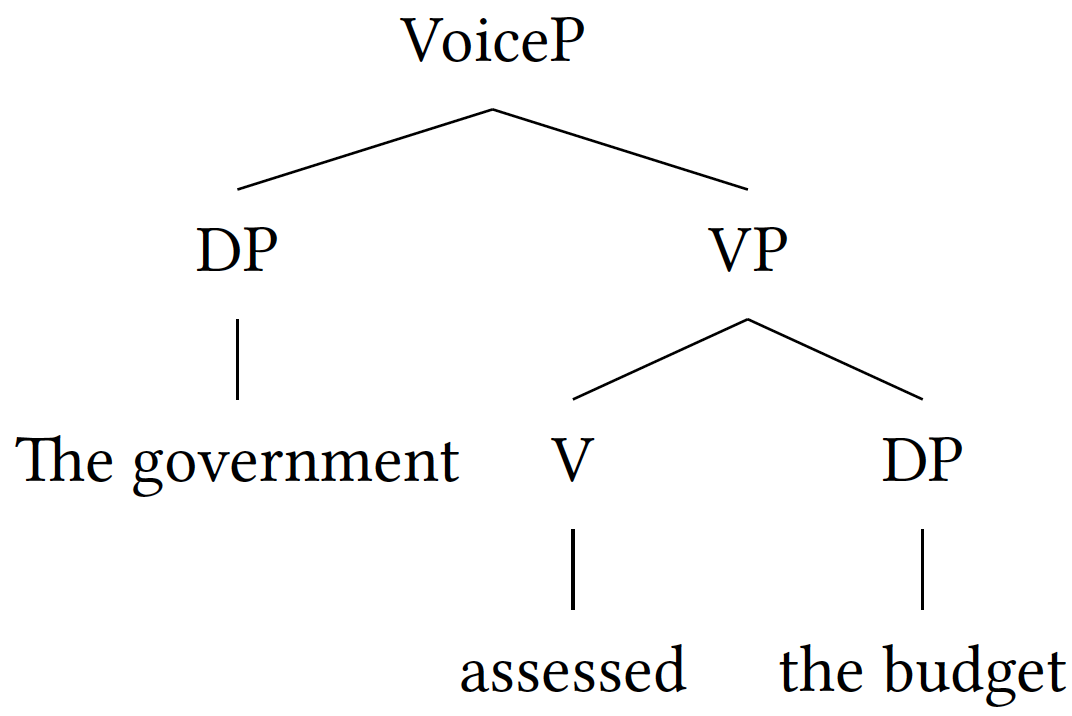
\includegraphics[width=0.55\linewidth]{figures/ex_forest}
    \end{center}
% \begin{forest}%syll
% [VoiceP
% [DP[The government]]
% [VP
% [V[assessed]]
% [DP[the budget]]
% ]
% ]
% \end{forest}
}
\end{exe}

 {A DC based on the construction  in (\ref{tree}) contains \textit{two} nouns: one is the head derived from the verb and the other is the non-head. The latter can realize only one of the two arguments of the verb. Given the hierarchical structure in (\ref{tree}), this must be the object: see \textit{budget assessment}. Nothing prevents the original subject to be realized as a non-head (e.g., \textit{government assessment}). In that case, however, the DC does not follow the compositional make-up in (\ref{tree}), since the object is missing and the subject cannot form a constituent with the transitive verb alone. Such a DC will be interpreted by means of world knowledge, similarly to RCs as in (\ref{2}). From this perspective, the  subject behaves just like an adjunct/modifier, since it does not play any role in the compositional make-up of the DC.}\footnote{Indirect objects are included here as well, since they also attach to the verb after the direct object does: see \cite{larson:88}.}

 The importance of compositionality in language use is undebatable: without recursive compositional rules, speakers would not be able to produce and understand infinitely many sentences (\cite{dowty:07}). That compositionality in DCs imposes an object interpretation, as predicted by the structure in (\ref{tree}), is supported by the fact that the default reading of a possibly ambiguous DC like \textit{police killing} is that with an object non-head; the subject reading becomes available if established by a particular context, as, e.g., recent discussion in the U.S.\ about police killing unarmed civilians. Similarly, out of context, \textit{student evaluation} also receives an object interpretation. The subject reading is brought about by a particular social environment in which people talk about students evaluating their teachers. Moreover, as shown in the linguistic literature (e.g., \cite{grimshaw:90,borer:13,iordachioaia:alexiadou:pairamidis:17}), if a DC type is  compositionally derived from a VP, it should also be fully productive: that is, any verb--object combination should be able to form a compositional DC, which is confirmed, for instance, by (\ref{subj:obj:dcs}b). By contrast, not any subject--verb combination can form a DC: the non-heads in  (\ref{subj:obj:dcs}c) may at best receive a peculiar object interpretation, but not the subject reading of the corresponding sentence in (\ref{subj:obj:dcs}a).

\begin{exe}
\ex{\label{subj:obj:dcs}\begin{xlist}
\ex A \textit{boy}/\textit{girl} broke the \textbf{window}/\textbf{pen}.
\ex \textbf{window} breaking, \textbf{pen} breaking 
\ex *\textit{boy} breaking, *\textit{girl} breaking
\end{xlist}
}
\end{exe}


To summarize, ambiguous DCs as in (\ref{5}) below are partially opaque, as the relationship between the two nouns is not explicit, and may receive several interpretations.
However, if the DC is interpreted compositionally (in parallel to the verbal construction), it will be fully transparent and involve an object reading. The task remains to find independent evidence for the compositionality of a DC. In this respect, we will follow \citeauthor{grimshaw:90}'s~(\citeyear{grimshaw:90}) distinction from \sectref{sec:lit:ASN:RN} concerning the head nouns of DCs, as specified below in \sectref{sec:intro:contribution} and \sectref{sec:theory:features}.

\begin{exe}
\ex{\label{5}
\begin{xlist}
\ex{policy/police/radio announcement \hfill (Object/Subject/Adjunct)}
\ex{marketing approval, security assistance \hfill (Object/Subject/Adjunct)}
\end{xlist}}
\end{exe}



\paragraph*{Terminology}
 Before we introduce our research program, a few terminological clarifications are in place. The term \textit{compositionality} is often used without particular focus on the syntactic-semantic relationship between the parts of the complex expression, an aspect that is of crucial importance in our study. Natural Language Processing literature on (root) noun-noun compounds, for instance, occasionally speaks of \textit{compositionality ratings}, in which annotators evaluate how accessible the lexical meaning of the two nouns is in the overall meaning of the compound (see \sectref{sec:NLP:lit:compositional} for details and references). This notion of compositionality is similar to what we call below \textit{lexico-semantic transparency}.

 A notion of \textit{compositionality} that is closer to ours appears in some Distributional Semantics (DS) approaches, which, in view of the PoC in (\ref{3}), seek to identify linguistically-informed composite functions to combine the individual parts of complex expressions (e.g., \cite{marelli:baroni:15,baroni:zamparelli:10}). Like us, these authors take a closer look at the relationship between the parts; however, their focus is more on the technical implementation (i.e., the DS correspondent of function application from theoretical linguistics) rather than on the linguistically relevant constraints that are at play. Although we share the interest in the relationship between the parts with this literature, we are not concerned with the technical details of the function, but with how this relationship interacts with other morphosyntactic properties of the head, as explained in \sectref{sec:intro:contribution}.

We use the terminology as follows: \textit{compositional} refers to DCs that encode the structure in (\ref{tree}). Some may call this \lq syntactic compositionality\rq. The term \textit{transparent} is broader and allows two specifications. First,  \textit{lexico-semantically transparent}  characterizes the compounds whose parts are semantically fully recoverable from the compound meaning. These include all DCs as in (\ref{1}) and (\ref{5}), as well as some RCs as those in (\ref{2}).\footnote{Other RCs like \textit{hogwash} are substantially less transparent: see the previous literature in \sectref{sec:NLP:lit}.}  Second, 
what we would call \textit{compositionally transparent} applies to DCs that, besides being lexico-semantically transparent, also follow the structure in (\ref{tree}). These correspond to our \textit{compositional DCs}, since all the DCs we consider here are lexico-semantically transparent.



\subsection{Our contribution}\label{sec:intro:contribution}
 We start with the assumption that an important source of ambiguity  in DCs such as in (\ref{5}) is the ambiguity of their deverbal head nouns as in (\ref{6}) and the correlated ambiguous relationship that they establish with the non-heads.  The non-head is entirely transparent in DCs: its lexical semantics is present in the DC meaning, and, as an argument or adjunct, it brings no syntactic constraints to influence its syntactic-semantic relationship with the head noun. By contrast, the head noun is more complex. Its lexical semantics is also visible in the DC; yet, following Grimshaw's distinction in (\ref{6}), its ambiguity between ASN and RN readings has a great impact on its syntactic-semantic relationship with the non-head. As perfect  transpositions of verb phrases, ASNs follow the compositional structure in (\ref{tree}) and require objects to be realized first. RNs maintain only remote lexical connections to the verb base and do not inherit their compositional structure. Thus, RNs impose no syntactic requirements on the non-heads and are compatible with any syntactic-semantic relationship allowed by their lexical semantics.


 Following this reasoning, our hypothesis is that DCs with ASN heads will obey the constituent structure  in (\ref{tree}) and realize only objects as non-heads. These DCs will be both compositional  and lexico-semantically transparent. DCs whose heads are RNs  do not respect this structural condition and allow any interpretation that a context  or world knowledge provide -- whether related to the base verb or not  (cf. \textit{police building} \lq building that hosts the police department\rq). In this respect, DCs headed by RNs are semantically similar to RCs; their deverbal morphology is irrelevant for their interpretation, since they are lexicalized.  Such DCs are lexico-semantically transparent, but they are not fully compositional.


To test this hypothesis, we  use a series of morphosyntactic properties that Grimshaw argued to be ASN-specific (see~$§$\ref{sec:theory:features})  and check their presence in the behavior of DC heads, on the basis of evidence from a large corpus of naturally occurring text.  
 Since it is not a given fact that the ASN-features defined by Grimshaw can be reliably informed by corpora, we also gathered human judgments on ASN-hood -- namely, we asked annotators to indicate in how far the deverbal head refers to a process (or verbal event). By asking annotators directly for their judgments, we try to get an estimate for the latent variable that underlies the ASN properties defined by Grimshaw. We use these different types of data as features in a logistic regression classifier, by which we aim to predict the syntactic-semantic relation between the head and the non-head.  These results are compared with the manually annotated interpretation of DCs. 
 

Given our hypothesis and methodology, we expect that the ASN-features extracted from the corpus, as well as that based on human judgments, will point to an object interpretation of the DC (as predicted by  (\ref{tree})) and will have high predictive power in determining whether the DC's non-head is an object or not. A high predictive power of the features will additionally show us that compositionality is an important aspect in the disambiguation of DCs.

First of all, our results indicate that all the ASN-hood features have predictive power above the chance level when tested individually and  together. The most stable individual features point to an object interpretation, as expected under our hypothesis. Second, the ablation experiments  show that many features overlap in the identification of ASN-hood, inviting to theoretical reflection on  the individual contribution of these features. Third, the best feature is the manual annotation of ASN-hood,  which confirms the importance of this property for interpreting DCs;  it also indicates that either the morphosyntactic features are comparably weaker or our corpus did not offer enough material for better results. Fourth, some weaker features raise stimulating questions especially relevant for linguistic investigation.

 Our study investigates transparency strictly from the perspective of the compositional structure in  (\ref{tree}). The degree of (lexico-semantic) transparency of DCs that do not receive such a verb-related compositional interpretation (i.e., those headed by RNs) goes beyond the scope of our present study and must be left for a future endeavor. As mentioned above, the role of world knowledge and context is essential for such DCs. Therefore, such an investigation would need to employ a different methodology, more similar to that pursued in several computational studies as presented in  ~\sectref{sec:NLP:lit:compositional}. We also do not aim to measure speaker intuitions about the transparency degrees of DCs (as done in some of these computational approaches), although it would be interesting to compare such ratings with our relation-based annotations  in the future. Our present study conceptually differs from these computational approaches, as it addresses the transparency of DCs from a structural perspective. We use insights from theoretical linguistics on the morphosyntactic properties of the deverbal noun heads of DCs and general principles of syntax-semantics mapping, and test these theoretical hypotheses  with corpus-based and computational methods.

We start with an overview of relevant  {previous studies from Theoretical Linguistics (TL)} and  {Natural Language Processing~(NLP)} in \sectref{sec:previous:lit}.
Sections \sectref{sec:methodology} and \sectref{sec:features} describe our data collection and methodology; \sectref{sec:ML} presents our experiments, followed by a discussion in \sectref{sec:discussion}. We draw our conclusions in \sectref{sec:conclusions}.






\section{Previous literature}\label{sec:previous:lit}
In \sectref{sec:theoretical:lit} we introduce the main theoretical concepts  that have guided our investigation and briefly refer to previous analyses of DCs relevant to our assumptions. \sectref{sec:NLP:lit} presents the  {NLP} literature on  {deverbal and root} noun-noun compounds and the extent to which these studies can be compared with ours.

\subsection{Theoretical approaches to DCs}\label{sec:theoretical:lit}
Deverbal compounds have been at the forefront of theoretical linguistics since the early days of generative grammar. Especially beginning with the 70s, after \citeauthor{chomsky:70}'s~(\citeyear{chomsky:70}) \textit{Remarks on nominalization}, the theme of the theoretical debate has been whether word formation is part of the syntax or the lexicon. Syntactic approaches have argued that DCs behave systematically enough to be accounted for by syntactic rules (e.g., \cite{roeper:siegel:78,ackema:neeleman:04}); lexicalist approaches have pointed out peculiar properties of DCs, which would require their analysis as part of the lexicon (e.g., \cite{selkirk:82,lieber:04}). 

The syntax vs. lexicon debate is relevant for our study in so far as recognizing a syntactic component in DCs leads to their compositional analysis, while specifying lexical rules for them suggests that they are like RCs and lack a systematic morphosyntax that preserves phrase-like compositionality. Meanwhile, both theoretical trends have argued for both kinds of analysis of DCs, and we will abstract away from the type of framework to focus on the properties of DCs.


Noteworthily, in theoretical studies the problem of compositionality in DCs is not addressed with respect to the contribution of the two individual nouns as in recent NLP studies (see~\sectref{sec:NLP:lit}). If available at all, implications on compositionality come indirectly from the claims on the  make-up of DCs and the structural relationship between their  parts as in (\ref{tree}) (see~\sectref{sec:prev:lit:DCs}).

\subsubsection{Morphosyntactic properties of ASNs}\label{sec:properties:ASN}
 In support of the contrast illustrated in~(\ref{6}), \cite{grimshaw:90}  argues that  deverbal nouns in their ASN reading exhibit a special morphosyntactic behavior, which is not shared by RNs.
\tabref{tab:1:ASN:RN} is a summary of the main contrastive properties of ASNs (vs.~RNs) from \cite{grimshaw:90} that are relevant for our study, adapted from \citet[3]{alexiadou:grimshaw:08}.\  These properties are positively specified for ASNs only, since RNs behave like non-derived lexical nouns and do not present any such particularities. The reasoning is that ASNs have  verbal properties (i.e., event structure as in (\ref{tree})), which will impose restrictions on their nominal behavior (e.g., must  appear in the singular) or make them compatible with verb-specific modifiers (e.g., aspectual adverbials).

\begin{table}
\caption{Morphosyntactic properties of ASNs vs.\ RNs }
\label{tab:1:ASN:RN}
\begin{tabular}{|l|l|l|l|}
\hline & \textbf{Morphosyntactic property} & \textbf{ASN} & \textbf{RN}\\ \hline
i. & Obligatory object arguments realized as \textit{of}-phrases & Yes & No \\ \hline
ii. & Agent-oriented modifiers (\textit{deliberate}, \textit{intentional}, \textit{careful}) & Yes & No\\ \hline
iii. & \textit{By}-phrases are (subject) arguments &Yes & No\\ 
\hline
iv. & Aspectual \textit{in}/\textit{for-X-time} adverbials & Yes & No\\ \hline
v. &  \textit{Frequent}, \textit{constant} appear with singular & Yes & No\\ \hline
vi. & Must appear in the singular & Yes & No\\
\hline
\end{tabular}
\end{table}

 The realization of object arguments is a necessary and sufficient condition for ASNs.\ It indicates the presence of verbal event structure, which associates with the other ASN-properties. However, the morphosyntactic means to introduce an object argument in nominals is an \textit{of}-phrase, which may also express possession. Given this ambiguity, using an  \textit{of}-phrase in combination with other ASN-properties is more reliable. For instance, in  (\ref{6}b), the predicate \textit{took a long time} requires an event as a subject, which shows that \textit{the examination of the patients} is an ASN, while \textit{the exam of the patients} is not.
As mentioned above, in the latter case \textit{of the patients} expresses a possessor of the entity \textit{exam}.

Agent-oriented adjectives like \textit{deliberate, intentional, careful} are also taken by \citet[51--52]{grimshaw:90} to depict ASNs.  Like \textit{of}-phrases, possessive marking is ambiguous between expressing subject arguments, as in (\ref{ex:agentive}b), and possessive modifiers,  as in (\ref{ex:agentive}c)). Agentive modifiers, however, require verbal event structure with a subject (agent) argument, which cannot be available in the absence of the object argument in (\ref{ex:agentive}a) and (\ref{ex:agentive}c)) (cf.~the hierarchy in (\ref{tree})). The contrast between (\ref{ex:agentive}a) and (\ref{ex:agentive}b) shows that the possessive \textit{the instructor's} cannot introduce the subject argument, if the object argument is not realized.

\begin{exe}
\ex{\label{ex:agentive}
\begin{xlist}
\ex{*The instructor's \textit{intentional/deliberate} examination took a long time.}
\ex{The instructor's \textit{intentional/deliberate} examination \textit{of the papers} took a long time.\hfill (ASN)}
\ex{the instructor's (\textit{*intentional/*deliberate}) book}
\end{xlist}}
\end{exe}

 In ASNs, \textit{by}-phrases have a function similar to that of the possessive in (\ref{ex:agentive}b): they introduce the subject argument. Yet, like the possessive and \textit{of}-phrases, \textit{by}-phrases may also introduce modifiers. In (\ref{ex:by}a), the \textit{by}-phrase acts as a modifier of the lexical noun \textit{book}, which has no event structure. In (\ref{ex:by}b), however, it introduces the subject argument of an ASN, the same way the possessive does in (\ref{ex:agentive}b). (\ref{ex:by}c) is ungrammatical, because the agent-oriented modifiers \textit{intentional/deliberate} require a subject argument, which the \textit{by}-phrase cannot introduce in the absence of event structure and the object: (\ref{ex:by}c) parallels (\ref{ex:agentive}a).

\begin{exe}
\ex{\label{ex:by}
\begin{xlist}
\ex{a book \textit{by Chomsky}}
\ex{The intentional/deliberate examination \textit{of the papers} \textit{by the instructor} took a long time.\hfill (ASN)}
\ex{*The intentional/deliberate examination \textit{by the instructor} took a long time.}
\end{xlist}}
\end{exe}

 {Given the verbal event structure and the correlated aspectual properties of ASNs, they are expected to allow aspectual adverbials and to obey the aspectual restrictions of their base verbs. In (\ref{ex:aspect}a), the telic verb \textit{destroy} allows \textit{in}- but not \textit{for}-adverbials. The correlated ASN in (\ref{ex:aspect}b) exhibits the same constraint. By contrast,  simple nouns that lexically denote events such as \textit{trip, process} are incompatible with such modifiers in (\ref{ex:aspect}c), although they occupy time, as shown by (\ref{ex:aspect}d). The latter pattern with RNs \parencite[58--59]{grimshaw:90}.}

\begin{exe}
\ex{\label{ex:aspect}
\begin{xlist}
\ex{The bombing destroyed the city \textit{in/*for only 2 days}.}
\ex{The total destruction of the city \textit{in/*for only 2 days} appalled everyone.}
\ex{*The process/John's trip \textit{in/for 5 hours}}
\ex{The process/John's trip \textit{took 5 hours}.}
\end{xlist}}
\end{exe}

 {Finally, Grimshaw argues that, due to their verbal structure, ASNs, in general, disallow plural marking, and when plural is available it indicates a RN reading. This is illustrated in (\ref{ex:plural}) from \citet[54]{grimshaw:90}. Related to this and the aspectual contrast in (\ref{ex:aspect}), Grimshaw notes that aspectual modifiers like \textit{constant, frequent} will combine with a singular ASN, but with a plural RN. These modifiers require habitual/iterative aspect, which is made available by the event structure of ASNs, but not by the lexicalized RNs. The latter need the plural to contribute the iterative meaning: see (\ref{ex:constant}a)/(\ref{ex:constant}c)--(\ref{ex:constant}b).}

\begin{exe}
\ex{\label{ex:plural}
\begin{xlist}
\ex{The \textit{assignments} were long.\hfill (RN)}
\ex{*The \textit{assignments of the problems} took a long time.\hfill (ASN)}
\ex{The \textit{assignment of that problem} always causes problems.\hfill (ASN)}
\end{xlist}}
\end{exe}

\begin{exe}
\ex{\label{ex:constant}
\begin{xlist}
\ex{*The \textit{constant} assignment is to be avoided.\hfill (RN)}
\ex{The \textit{constant} assignment of unsolvable problems is to be avoided.\hfill (ASN)}
\ex{The \textit{constant} assignment\textbf{s} were avoided by students.\hfill (RN)}
\end{xlist}}
\end{exe}

 {In (\ref{ex:agentive}) to (\ref{ex:constant}), the contrasts between ASNs and RNs are clear. Yet, depending on the lexical semantics of the individual nouns, the application of these tests may exhibit quite a bit of variation, which led many to challenge Grimshaw's generalizations. For instance, \cite{alexiadou:iordachioaia:soare:10} show that in some languages, ASNs may pluralize provided particular aspectual properties, while  \cite{grimm:mcnally:13} and \cite{lieber:16} challenge some of Grimshaw's claims with counterexamples attested in corpora. However, a general tendency of ASNs to exhibit the properties in Table~\ref{tab:1:ASN:RN} cannot be denied. At least so far, no corpus study has offered a quantitative analysis to prove that these properties are irrelevant for ASNs. From this perspective, our study can also be viewed as testing the relevance of these properties on the basis of deverbal compounds, which, according to Grimshaw, are headed by ASNs (see \sectref{sec:prev:lit:DCs}).}


\subsubsection{Deverbal compounds between ASNs and RNs: \cite{grimshaw:90}}\label{sec:prev:lit:DCs}
Let us now consider DCs from the perspective of the documented ASN vs.\ RN contrast. We focus  on Grimshaw's analysis of DCs and on \cite{borer:13}, the latter of which reviews Grimshaw's arguments to support an opposite position.

In her study of nominalization, \cite{grimshaw:90} argues that the heads of DCs (i.e., her \textit{synthetic compounds})  are ASNs.  Her reasoning relies on the observation that DCs obey argument structure constraints in the realization of their non-heads. In her  model of argument realization, she proposes a hierarchy of argument roles as in~(\ref{7}), such that the lower arguments (from right to left) must be realized syntactically before the higher ones.
This means that the theme, i.e., the syntactic direct object, must be realized before the goal (indirect object) and the agent (subject).  {This thematic hierarchy reminds us of the constituent structure of verb phrases in (\ref{tree}).}

\begin{exe}
\ex{\label{7} Agent (subject) > Goal (indirect object) > Theme (direct object)}
\end{exe}

Grimshaw argues that DCs obey the hierarchy in (\ref{7}), since they disallow non-heads that realize other arguments than the theme (object). (\ref{8}) repeats two of her examples. Her explanation is that, when occurring in DCs, deverbal nouns such as  \textit{giving} and \textit{reading} are disambiguated to an ASN interpretation. 
\begin{exe}
\ex{\label{8}
\begin{xlist}
\ex[]{They give \textbf{gifts} to \textit{children}. \\
DC: \textbf{gift}-giving to children vs.\ *\textit{child}-giving of gifts}
\ex[]{\textit{Students} read \textbf{books}.\\
DC: \textbf{book}-reading by students vs.\ *\textit{student}-reading of books}
\end{xlist}}
\end{exe}
In contrast to suffix-based deverbal nouns as in (\ref{8}), she considers zero-derived nouns like \textit{a sting} and \textit{a bite} to always be RNs. She shows that the compounds these may head need not obey the hierarchy in~(\ref{7}) and allow agent non-heads. The grammatical compounds in~(\ref{9}) are RCs for Grimshaw. 
\begin{exe}
\ex{\label{9} \textbf{bee} sting (vs. *bee-stinging), \textbf{dog} bite (vs. *dog-biting)}
\end{exe}

\subsubsection{Deverbal compounds between ASNs and RNs: \cite{borer:13}}
In spite of her extensive study on ASNs, Grimshaw does not go to great lengths to compare DCs with ASNs in terms of  morphosyntactic properties such as those in \tabref{tab:1:ASN:RN}. \cite{disciullo:92} investigates some of these tests in further support of the similarity between DC heads and ASNs. However, two decades later, \cite{borer:13} challenges Grimshaw's analysis of DCs by using some of these morphosyntactic tests. She argues that the behavior of DCs essentially differs from that of ASNs, and proposes that all DCs are headed by RNs.

We retain three of Borer's arguments.
First, she argues that, unlike ASNs, DCs disallow aspectual \textit{in}/\textit{for}-adverbials and, second, that they also disallow argumental \textit{by}-phrases.
This contrast is illustrated in (\ref{10})  {(cf.\ (\ref{ex:aspect}) and (\ref{ex:by}))}.
In Borer's system, the unavailability of aspectual modifiers indicates that event structure (with arguments) is entirely missing from DCs, so they cannot involve ASNs.\ Her conclusion is that DCs are headed by RNs and behave just like RCs. 

\begin{exe}
\ex[]{\label{10} 
\begin{xlist}
\ex[]{the demolition of the house \textbf{by the army} \textit{in 2 hours}\hfill (ASN)}
\ex[]{the  {stabbing} of the emperor \textbf{by Brutus} \textit{for 10 minutes}\hfill (ASN)}
\ex[]{the house demolition (*\textbf{by the army}) (*\textit{in 2 hours})\hfill (DC)}
\ex[]{the emperor  {stabbing} (*\textbf{by Brutus}) (*\textit{for 10 minutes})\hfill (DC)}
\end{xlist}}
\end{exe}

Third, Borer claims that the object reading of non-heads in DCs is just as available as a subject reading, depending on context.
As evidence, she quotes DCs  as in~(\ref{11}), parallel to those in~(\ref{1}b), whose non-heads may correspond to subjects. 

\begin{exe}
\ex[]{\label{11} teacher recommendation, court investigation, government decision}
\end{exe}

Some criticism and re-interpretation of Borer's facts is found in \cite{iordachioaia:alexiadou:pairamidis:17} and \cite{iordachioaia:toappear}.
We briefly note here that aspectual adverbials are barely ever attested in corpora even with ASNs \citep[39--42]{lieber:16}, so an extensive empirical study is necessary to determine how much DCs differ from ASNs in this respect.
Furthermore, \textit{by}-phrases are broadly attested with DCs in corpora, as Grimshaw's~(\ref{8}b) also predicts, but they usually involve bare plurals and not definite noun phrases or proper names as in Borer's~(\ref{10}c-d).
Given that DCs are often generic, this restriction is natural.

Having summarized these two  theoretical approaches to DCs, we may add that we do not aim to argue for one or the other. Instead, we use morphosyntactic properties whose pertinence for ASN-hood is accepted by both to guide us in evaluating the impact of the head noun on the interpretation of the DC. Our hypothesis that a high level of ASN-hood in DC heads correlates with an object reading of the non-heads, however, follows Grimshaw's intuition that \lq true\rq\  DCs involve ASN heads and are fully compositional. By contrast, Borer's claim is that DCs are always ambiguous like RCs and never as compositional as ASNs.
 {Given that our results support the correlation between ASN-properties and an object reading in DCs, they also bring some evidence against Borer's analysis.}

\subsection{Computational approaches to compounds}\label{sec:NLP:lit}
Compounds have been the focus of quite a number of papers in the field of Computational Linguistics (CL) and NLP. In view of the topic of this paper there are two strands of research that are most relevant. The first  focuses on determining the relation between the two components of a compound, the head and the non-head. 
For our study this work is relevant to the extent that it discusses compounds whose head is a deverbal noun.  
The second strand of research is concerned with modeling the  {lexico-semantic transparency} of noun-noun compounds. We will start by discussing the former and finish with an overview of the work that predicts the degree of  {transparency} in compounds.

\subsubsection{Predicting the interpretation of  {deverbal} compounds}\label{sec:NLP:lit:predictions}
The goal of computational work on deverbal compounds (referred to as nominalizations) has been to predict the relation between the non-head and the deverbal head. The relation inventory  
has varied from two classes, OBJ and SUBJ, in~\cite{lapata:02}, to three classes, OBJ, SUBJ and prepositional complement in~\cite{NicholsonBaldwin:06}, and to 13 classes -- OBJ, SUBJ and further specifications of the prepositional complement in~\cite{grover:lapata:lascarides:05}. 

These works have mostly focused on encyclopedic, usage-based features such as the syntactic relations attested between the base verb of the head noun 
and the non-head in large corpora. The underlying assumption is that the frequency distribution of syntactic relations between a given noun and a verb, for example, between \textit{taxi} and \textit{drive}, is a good estimate for the distribution of the underlying relation between \textit{taxi} and \textit{driver}. Additional pragmatic knowledge is obtained  from the direct context of the compound.
In selecting these pragmatic features, these works are in line with lexicalist theoretical approaches that list several covert semantic relations typically available in compounds (cf.\ most notably, \cite{levi:78}, see~\cite{fokkens:07}, for a critical overview). In addition to these pragmatic features, some 
straightforward morphological features are selected, such as the suffix of non-heads ending in~\textit{-ee} and~\textit{-er}~\citep{lapata:02}.

Our study differs from these works in several ways. First, our aim is not to reach state-of-the-art performance in prediction, but to  {test linguistic hypotheses by} measuring the predictive power of the various features discussed in theoretical linguistics, which are also indicative of the  {compositionality} of the compound. 

Second, and related to the previous point, our features are all head-specific. This is because,  following Grimshaw's theory, the behavior of the derived nominal heads (as~ASNs or~RNs) should mirror the structural correlation between DCs and the compositional structure of the original verb. The presence (or absence) of such a correlation is expected to have a great impact on the relation between the head and the non-head. In order to measure the individual impact of these theoretically-defined features, we do not rely on pragmatic features  {that involve both the head and the non-head} as in the studies above.
 

Lastly, because our goal is to uncover in how far the behavior of the derived nominals (as ASNs or RNs) can  predict the relation between head and non-head, we carefully selected  {equal numbers} of DCs with the suffixes \textit{-al}, \textit{-ance},  \textit{-ing},  \textit{-ion}, and  \textit{-ment}. These suffixes are all ambiguous in their formation of ASNs and RNs, so we eliminate any bias for particular readings (cf. \textit{-ee} and \textit{-er}, \sectref{sec:extraction:dcs}).

\subsubsection{Predicting  {the degree of transparency in noun-noun} compounds}\label{sec:NLP:lit:compositional}
For the transparency of  compounds two types of CL work are relevant,  {which} focus on different tasks, but share the same assumptions.\ One type  aims to predict the meaning of compounds based on composite functions between the vector-based representations of their parts, e.g.,~\cite{OSeaghdha:2008} and~\cite{Mitchell:2010}.
These works  compare different types of mathematical functions for the combination of the vectors for heads and non-heads to best represent the  meaning of compounds.  {In the same spirit, but closer to our interest in the syntactic-semantic relationship between the parts, \cite{marelli:baroni:15,baroni:zamparelli:10} investigate linguistically-informed composite functions.}

The other line of work aims to predict the degree of  {lexico-semantic transparency}  {(i.e., what they call \lq compositionality\rq; cf.~\sectref{sec:intro:compositionality})} of compounds {. For this, they compare} the vector-based representations of the parts and composite functions  {to} the vector-based representations of the compound as a whole, e.g., \cite{SchulteImWaldeEtAl:16,Reddy:2011}. 

This  second line of work also draws upon psycholinguistic insights,  such as~\citet{Libben:1997,Libben:2003}, which groups noun-noun compounds into four different categories, depending on the transparency of the head and the non-head.
The four classes are:
 {\textsc{tt}} for compounds with both a transparent head and non-head,
 {\textsc{oo}} for compounds with opaque heads and non-heads,
and  {\textsc{ot}} and  {\textsc{to}} for compounds whose parts differ along the dimension of transparency. They found that both semantically opaque and semantically transparent compounds show morphological constituency. However, they found the semantic transparency of the head to play a significant role. This confirms previous results from the psycholinguistic literature~(\cite{Zwitserlood:1994}). 

 {In this literature, several datasets have been created, which collect human ratings on the degrees of lexico-semantic transparency of compounds with respect to their constituents: e.g., in English~\citep{Reddy:2011,Juhaszetal:2015} and in German~\citep{SchulteImWaldeEtAl:16a}.} 
\cite{SchulteImWaldeEtAl:16a} have enriched the semantic transparency ratings with several empirical features related to the  {constituents} of the compound in order to measure the influence of these features on the  {transparency} of the compound. These features include:
\begin{itemize}
\item Corpus frequencies of the compounds and their parts;
\item Productivity of the parts, as in the number of compound types the part (head/non-head) appears in;
\item Number of senses for the parts as retrieved from GermaNet~\citep{hamp:97,heinrich:10} for the German dataset and WordNet~\citep{fellbaum:98} for the English dataset.
\end{itemize}

\cite{SchulteImWaldeEtAl:16} use vector space models to model the meaning of the compounds and their parts. Subsequently, they model the  {transparency} of the compound by measuring the distance between the composite vector of its parts and the vector for the actual compound. The assumption behind this work is that the vectors of  {transparent} compounds should be closer to the composite function of their vectors than the vectors of  {opaque} compounds. 

The main question \cite{SchulteImWaldeEtAl:16} try to answer  
is whether the above-mentioned properties (frequency of the compound and its parts, productivity, and ambiguity of its parts) play a major role in the  quality of the predictions. They found that for the head all properties had a significant effect on the predictions, whereas for the modifier the effect was not consistent. This converges with our results in predicting the compositionality of DCs from the properties of the head.

Furthermore, they attribute the influence of these features to the underlying  ambiguity that they seem to be correlated with: e.g., frequent heads that are highly productive are often highly ambiguous.  {We note, however, that these studies are not  concerned with DCs, as ours, but especially with what we call RCs, some of which are lexico-semantically less transparent than our DCs (cf.~\textit{hogwash}).}




\section{Methodology}\label{sec:methodology}
In this section we present the corpus and the tools for automatic pre-processing, the procedure in the DC extraction, as well as the annotation and post-processing of our collection of DCs.
\subsection{Corpus and tools}
For the selection of DCs and to gather corpus statistics on them, we exploited the Annotated Gigaword corpus~\citep{Napoles:12}, one of the largest general-domain English corpora, which contains several layers of linguistic annotation. This corpus encompasses ten million documents from seven news sources and more than four billion words.                                      
We made use of the following available automatic preprocessing steps and annotations, which we accessed via the Java API provided along with the corpus: sentence segmentation~\citep{Gillick:09}, tokenization, lemmatization and POS tags (Stanford's CoreNLP toolkit\footnote{http://nlp.stanford.edu/software/corenlp.shtml}), and constituency parses~\citep{Huang:10} converted to syntactic dependency trees with Stanford's CoreNLP toolkit.
The POS tags adhere to the Penn Treebank tagset~\citep{Santorini:93}; the dependency relations follow the Stanford typed dependencies~\citep{Marneffe:08}.
As news outlets often repeat news items in subsequent news streams, the corpus contains a considerable amount of duplication. To improve the reliability of our corpus counts,  we removed exact duplicate sentences within each of the 1010~corpus files, reducing the corpus size by 16\%.


\subsection{Extraction of deverbal compounds}\label{sec:extraction:dcs}
We created a balanced collection of DCs, which we extracted from the Gigaword corpus. We first gathered 25 nouns (over three frequency bands : high, medium, low) for each of the suffixes \textit{-al}, \textit{-ance}, \textit{-ion}, \textit{-ing}, and \textit{-ment}. The highest frequency band ranges from 4.5 to 3.5 on the Zipf-scale \citep{VanHeuven:2014}, the medium frequency band ranges from 3 to 2.5, and the lowest one from 2 to 1.5. 
The suffixes may form both ASNs and RNs according to \cite{grimshaw:90}. 


We  {did not} consider zero-derived nouns like \textit{attack}, \textit{abuse}, \textit{bite}, because Grimshaw considers them RNs~(see\ (\ref{9})).\ 
We also excluded deverbal nouns based on the suffixes~\mbox{\textit{-er}} and~\mbox{\textit{-ee}}, as they denote event participants corresponding to the subject and the object of the base verb, respectively, implicitly blocking this interpretation on the non-head~(cf.\ \textit{police$_{subj}$ train\textbf{ee}} -- \textit{dog$_{obj}$ train\textbf{er}}).\ In our attempt to capture the closeness of DCs to ASNs (and the base verbs), we considered only the suffixes that build eventive nominals, which could realize both a subject and an object argument. DCs headed by \textit{-ee} and \textit{-er} nouns would have been biased for one or the other. However, our selection of suffixes represents the large majority of deverbal nouns. They make up for 69.4\% of the total number of deverbal nouns in the NOMLEX database \citep{NOMLEX:98}, which consists of 1025 lexicalized deverbal nouns.


The nouns were selected such that their base verbs present transitive uses, making both subjects and objects available.\footnote{\textit{Arrive} is the only intransitive unaccusative verb that we used, which realizes the object/internal argument as a subject.} For illustration, \tabref{tab:2:nouns} offers  samples of deverbal nouns per each frequency range and suffix.\ For each such selected noun we then extracted the 25 most frequent compounds that they appeared as heads of, where available. A few deverbal nouns (in particular those with suffixes~\mbox{\textit{-al}} and~\mbox{\textit{-ance}}) were less productive in compounds and appeared with fewer than 25 different non-heads. Given these gaps and after removing a few repetitions due to capitalization, we obtained a collection of 3111 DCs.


\begin{table}\caption{\label{tab:2:nouns} Samples of extracted deverbal nouns}
{\footnotesize\begin{tabular}{|p{1.3cm}|l|l|l|l|l|}
\hline
 Frequency & AL & ANCE & (AT)ION & ING & MENT \\ \hline
%&spending & production & enforcement & proposal & insurance\\
High & approval & performance & protection & building & development \\
& withdrawal & assistance & reduction & training  & movement \\
%& bombing & construction & treatment & arrival & clearance\\
& rental & surveillance & consumption & trafficking  & punishment \\
\hline
% hearing & education & announcement & rehearsal & allowance\\
% laundering & exploration & payment & removal & maintenance\\
% testing & creation & imprisonment & disposal & resistance\\
%funding & prevention & assessment & reversal & guidance\\
% reading & registration & improvement & revival & attendance\\
Medium  & renewal & assurance & supervision & killing  & deployment\\
%& writing & destruction & replacement & burial & disturbance\\
 & survival & dominance & cultivation  & counseling & placement\\
%& firing & deprivation & assignment & denial & acceptance\\
 & upheaval & tolerance & instruction & teaching  & adjustment\\
%planting & examination & enrollment & dismissal & avoidance\\
%breeding & evacuation & enrichment & appraisal & remittance\\
%%growing & preservation & harassment & referral & acquaintance\\
%breaking & authorization & recruitment & refusal & inheritance\\
%learning & assassination & endorsement & deferral & resemblance\\
\hline
Low & retrieval & defiance & demolition & weighting & reinforcement \\
%&baking & anticipation & realignment & acquittal & reassurance\\
 & disapproval & endurance & expulsion & chasing  & empowerment\\
%& measuring & obstruction & mistreatment & rebuttal & remembrance\\
 & dispersal & ignorance & deportation & mongering & abandonment\\ 
\hline
\end{tabular}}
\end{table}

\subsection{Annotation and post-processing of DCs}\label{sec:annotation}
\subsubsection{Interpretation of (non-heads in) DCs}\label{sec:annotation:relation}
All DCs were annotated by three trained American English speakers, who had a university level background in  linguistics. They had to label the DCs as OBJ(ect), SUBJ(ect), OTHER, or ERROR, depending on the syntactic relationship that they considered the DC to establish between the base verb of the head noun and the non-head.
For instance, DCs such as in (\ref{1}) would be labeled as OBJ (\ref{1}a), SUBJ (\ref{1}b), and OTHER (\ref{1}c).
OTHER was an umbrella label for prepositional objects (e.g., \textit{adoption counseling} \lq somebody counsels somebody \textit{on adoption}\rq), various adjuncts (e.g., \textit{ultrasound examination} \lq to examine somebody \textit{with an ultrasound}\rq, \textit{sea burial} \lq to bury somebody \textit{by the sea}\rq, \textit{surprise arrival} \lq somebody/something arrived \textit{by surprise}\rq).
ERROR was  {intended} to identify errors of the POS tagger (e.g., \textit{face abandonment} originates in \lq they face$_V$ abandonment\rq), but was also employed by the annotators when they  considered the DC uninterpretable or  ungrammatical.
We allowed the annotators to use multiple labels and to indicate ambiguity (using~\lq --\rq) and the preferred order of the readings (using~\lq $>$\rq).

We used the original annotations to create a final list of compounds with the labels that all three annotators agreed on. 
For ambiguously labeled DCs we selected the one reading available for all three. 
If they all indicated the same ambiguity for a DC, we labeled the DC as ambiguous.\ 
The labels we used for the final dataset are OBJ, SUBJ, OTHER, DIS(agreement between annotators), AMBIG(uous), and ERROR.
In spite of \citeauthor{borer:13}'s (\citeyear{borer:13}) claims, we found only two cases of ambiguity which all three annotators agreed on -- namely, \textit{police killing} and \textit{doctor referral}, which were both labeled SUBJ--OBJ.
In the end we identified 772~DIS, 1377~OBJ, 404~OTHER, 286~SUBJ, and 273~ERROR cases of DCs.
After removing the disagreements, the two ambiguous DCs and the errors, we obtained 2067~DCs. We based our study on the agreed-upon relations only. We note, however, that the simple inter-annotator agreement (IAA) among the three annotators, excluding the errors, was 72.8\%. In a previous study with only two annotators~\citep{author:et:al:16}, the IAA was~81.5\%.

We kept two versions of the data: one in which  {the classes} OTHER and SUBJ are separate and one in which we conflated them to NOBJ (non-object). Given the purpose of this paper, i.e., verifying to what extent the OBJ reading of a DC correlates with particular morphosyntactic properties of the head noun, we focus here on the binary classification. The resulting data set is skewed with OBJ prevailing: 1377~OBJ and 690~NOBJ.

\subsubsection{Process vs.\ result readings in DCs}\label{sec:annotation:p-r}
An additional annotation task concerned feature 7.~\textit{process-vs-result} from~\tabref{tab:3:features} in \sectref{sec:theory:features} {. This feature} was designed to capture the three annotators' judgments with respect to how close the interpretation of the DC comes to the ASN and the verbal expression of a process/event in which the non-head is realized as SUBJ, OBJ, or OTHER.
They had to rate DCs from 5~(very prominent process) to~1~(no process = result)~(see~\cite{grimshaw:90}). 

We first explained to them the difference between an ASN and an RN as follows: ``\textit{The teacher's \textbf{assignment} of tasks} expresses a process in which the teacher assigns tasks.
However, in \textit{this long \textbf{assignment} took several hours to complete}, the noun \textit{assignment} is interpreted as a result of the process of assigning something -- namely, the task itself.''
We then instructed the annotators to check this contrast in DCs like \textit{task assignment} and \textit{Math assignment} and rate the ones that relate to the process as closer to~5 and those that relate to the result as closer to~1. Another example was \textit{apartment building}, which should be rated as closer to~5, if they interpret it as \lq to build apartments\rq, and closer to~1, if they  interpret it as \lq a building with apartments\rq. We fully encouraged the annotators to employ the scores 4, 3, 2 for unclear cases. 
 
During this task, the annotators had access to their previous  {SUBJ/OBJ/OTHER annotation} labels  for each DC and could compare different DCs headed by the same head noun. In terms of the variation of ratings between DCs headed by the same noun, one annotator in particular assigned pretty similar scores, although the contrast was clear. This annotator also showed a  tendency towards the extremes: either 5 or 1. In general, the task was perceived as difficult, especially by this annotator. We multiplied the scores from 5~to~1 by~20 to use them as percentages. For each DC we calculated the average between the three annotations obtaining values between~20 and~100. 
 
 
\section{The selection of morphosyntactic features}\label{sec:features}
\subsection{Theoretical considerations}\label{sec:theory:features}
To collect information on the morphosyntactic properties of the head nouns in DCs, we defined a total of nine morphosyntactic features, given in \tabref{tab:3:features}. 



\begin{table}\caption{\label{tab:3:features} Indicative features for head nouns}
{\footnotesize \begin{tabular}{|l|l|}
\hline  \textbf{Feature label} & \textbf{Description and illustration}\\ \hline
1.\ \textit{{\em of}\_outside\_DC} & Percentage of the head's occurrences as singular  outside compounds  \\ \citep{grimshaw:90}  & which realize a  syntactic relation with an \textit{of}-phrase. \\ & e.g., \textit{assignment \textbf{of} problems}\\ \hline
2.\ \textit{{\em by}\_outside\_DC} & Percentage of the head's occurrences in the singular  outside compounds  \\ \citep{grimshaw:90} &  which realize a  syntactic relation with a \textit{by}-phrase.\\ &   e.g., \textit{assignment (of problems) \textbf{by} teachers}\\ \hline
3.\ \textit{sum\_adjectives} & Percentage of the head's occurrences in a modifier relation with one \\ \citep{grimshaw:90}  &  of the adjectives \textit{frequent},  \textit{constant}, \textit{intentional}, \textit{deliberate}, or \textit{careful}.\\ 
\hline
4.\ \textit{sg\_outside\_DC} &  Percentage of the head's occurrences as singular outside compounds.\\ 
\citep{grimshaw:90} &\\
\hline
\hline
5.\ \textit{{\em by}\_inside\_DC} & Percentage of the head's occurrences as singular inside compounds  \\ ($\approx$ 2.~\textit{{\em by}\_outside\_DC}) & which realize a  syntactic relation with a \textit{by}-phrase.\\  &  e.g., \textit{task assignment \textbf{by} teachers}\\ \hline
6.\ \textit{sg\_inside\_DC} & Percentage of the head's occurrences as singular inside compounds.\\ 
($\approx$ 4.~\textit{sg\_outside\_DC}) & \\ \hline
7.\ \textit{process-vs-result}& Native speaker annotation of each DC as a process (\textit{car driving}) or  \\ ($\approx$ ASN vs.~RN) & result (\textit{apartment building})  on a scale from 5 to 1.\\
\hline
\hline 
8.\ \textit{suffix} & Suffix of the head noun: AL (rent\textbf{al}), ANCE (insur\textbf{ance}),\\ NEW & 
ING (kill\textbf{ing}), ION (destruct\textbf{ion}), MENT (treat\textbf{ment})\\ \hline
9.\ \textit{head\_in\_DC} & Percentage of the head's occurrences within a compound out of its \\  NEW &  total occurrences in the corpus.\\ \hline
\end{tabular}}
\end{table}


The first seven features are inspired by \cite{grimshaw:90},  {although only the first four directly correspond to the properties in \sectref{sec:properties:ASN}. Two adjustments led us to four features instead of the six properties in~\tabref{tab:1:ASN:RN}: first, \textit{in}/\textit{for}-adverbials were discarded, because we found close to no relevant data; second, we counted agent-oriented and aspectual adjectives together, as they were also very few.}\footnote{We initially collected data on \textit{in}- and \textit{for}-adverbials, but only a few nouns had such occurrences. At closer inspection even these examples turned out not to illustrate \textit{in}- and \textit{for}-phrases that modify the telic/atelic aspect of the head noun, as Grimshaw and Borer used them. Instead, they mostly functioned as temporal modifiers, and we therefore discarded this feature.}  In line with our hypothesis, we expect all these seven features to have predictive power and to point to an OBJ interpretation of the DCs.

Feature~1.~\textit{of\_outside\_DC} encodes the first property in~\tabref{tab:1:ASN:RN}. Here we counted the percentage of occurrences of a (singular) head noun in which it also realizes an  \textit{of}-phrase. For feature~2.~\textit{by\_outside\_DC} (i.e., third property in~\tabref{tab:1:ASN:RN}), we collected the frequency of a \textit{by}-phrase with a head noun. 
 Feature~3.~\textit{sum\_adjectives} collects all the (singular form) occurrences of the head nouns in a modifier relation with agent-oriented or aspectual adjectives (cf.~second and fifth property in~\tabref{tab:1:ASN:RN}).\footnote{Note that, given Grimshaw's assumption that ASNs do not appear in the plural, we counted all of these occurrences in the singular form of the head noun.} Feature~4.~\textit{sg\_outside\_DC} measures the percentage of singular occurrences of the head noun out of its total occurrences in the corpus  {(cf.~last property in~\tabref{tab:1:ASN:RN})}. 

Grimshaw's properties in \tabref{tab:1:ASN:RN} characterize deverbal nouns as ASNs when they appear on their own, i.e., \textit{outside} compounds. This is why features 1.~to 4.~are labeled correspondingly. Yet, if DCs are supposed to resemble ASNs, we considered that their head nouns should preserve these properties also within DCs, i.e., when the head noun is \textit{inside} a DC.\footnote{\cite{disciullo:92} and \cite{borer:13} actually apply the same reasoning.} For this reason, we also introduced the features 5.~\textit{sg\_inside\_DC} and 6.~\textit{by\_inside\_DC}. The former measures the percentage of singular DCs out of their total occurrences, and the latter the percentage of DCs that realize a \textit{by}-phrase. We did not test \textit{of}-phrases inside DCs, since DCs usually realize the object as a non-head (see our annotation results in \sectref{sec:annotation:relation}) and collecting such occurrences would have mostly delivered noise. The adjectives modifying DCs were also left out, because their number was close to inexistent.

There are two caveats to these corpus-based features inspired by \cite{grimshaw:90}. First, as we noted in \sectref{sec:properties:ASN}, the individual ASN-properties are not fully reliable in determining ASN-hood: e.g., there is ambiguity in argument marking (i.e., \textit{of}- and \textit{by}-phrases), and  deverbal nouns are easily coerced between the readings. For this reason, Grimshaw used several such properties together in her examples. However, we extracted these data from corpora, and most of the attestations were too few to allow any combined patterns beyond the one we ensured -- that of a singular form of the head noun in each of the other properties. Second, and related to this, basing our study on a corpus comes with the risk that, no matter how large the corpus, it may not present enough relevant data. It was for these two reasons that we considered adding three more head-related features to our study. We first gathered native-speaker intuitions about the ASN vs.~RN status of the head nouns in DCs (see  feature~7.~\textit{process-vs-result}) and supplemented Grimshaw's tests with information about the suffix  and the frequency of  the head noun within compounds (features~8.~\textit{suffix} and 9.~\textit{head\_in\_DC}).

We designed feature~7.~\textit{process-vs-result} (P-R) in order to grasp Grimshaw's intuition about the contrast between ASNs and RNs by means of introspection. The process vs. result interpretation is  the fundamental difference between ASNs and RNs in Grimshaw's understanding.   It can be seen as the latent variable that her morphosyntactic properties are intended to identify: ASNs express processes or events like the corresponding verbs, while RNs depart from this meaning and express results. Following this annotation (see~\sectref{sec:annotation:p-r}), we gathered information on how salient the verbal process is in the meaning of a DC and, indirectly, how accessible the compositional structure of the base VP is within the DC.\footnote{The way we gathered estimates for our P-R feature comes close to the NLP studies which gather native speaker evaluations about the transparency of compounds. Namely, our three annotators had to evaluate how close the morphosyntactic (and semantic) relationship between the head noun and the non-head comes to the fully compositional relationship between the corresponding verb and its argument or adjunct.}


The last two features~8.~\textit{suffix} and 9.~\textit{head\_in\_DC} represent two further properties of the head nouns that we considered interesting for our study. The theoretical literature does not offer much on suffixes. \textit{-Ing} has received most attention, to the extent that Grimshaw argued that it always forms ASNs, while Borer claims that it encodes  {what she calls an} originator (i.e., subject argument), with the effect that in compounds, the SUBJ reading is blocked for non-heads and OBj is favored. Neither contention is true. First, \textit{-ing} presents several examples of RNs (see~\textit{building(s)}, \textit{writing(s)}, \textit{reading(s)}).
Second, we \textit{do} find SUBJ-DCs headed by \textit{ing}-nouns (see~(\ref{1}b)). In general, the information on the suffix is independent of ASN-hood, since all suffixes allow both ASN and RN readings, but we aimed to check whether some suffixes may be more informative than others. 


Feature~9.~\textit{head\_in\_DC}~delivers us the degree of compoundhood of a deverbal noun, i.e., how likely it is to appear within a compound.
The expectation is that a noun that typically appears in compounds has undergone some meaning specialization, which requires another noun to be instantiated. One may rightly say that this makes the meaning of such head nouns less transparent than for those that freely appear both within and outside compounds. However, for deverbal nouns, to the extent that this slight meaning specialization requires a particular type of non-head, it can give us useful information about which (morpho)syntactic relationship between the base verb and one of its arguments is most likely to form a DC. If it is a non-OBJ relation, this shows that compositionality as in (\ref{tree}) is not a typical condition in the formation of DCs, weakening the relevance of our investigation. However, our results 
in Table~\ref{tab:prediction:all} below indicate that high compoundhood correlates with an OBJ interpretation of the non-head, which supports the relevance of compositionality in the formation of DCs.


\subsection{Technical support}\label{sec:technical:features}

To obtain statistics for the morphosyntactic features, we extracted counts for the selected DCs and their head nouns from the Gigaword corpus by matching patterns defined over word forms, lemmas, POS~tags and dependency relations, as provided by the automatic corpus annotations.
The specific patterns used for each feature are detailed in the following.

For the \textit{inside\_DC} features we extracted DCs from the Gigaword corpus by locating two adjacent nouns according to the POS~tags~NN for singular nouns and NNS for plural nouns, and  {excluding noun pairs directly preceded or succeeded by other} nouns or proper nouns (POS~tags NNP and NNPS). DCs were matched with the word form of the non-head and the lemma of the head, thereby extracting singular and plural occurrences.
We determined the grammatical number of a noun or compound by its POS~tag or the POS~tag of its head, respectively.
For example, we matched \emph{security training(s)}, but not \emph{airport security training} and \emph{security training instructor}, to make sure that we do not extract parts of larger compounds. Conversely,  the \textit{outside\_DC} features apply to head nouns (matched by their lemma and POS~tag NN or NNS) without any noun or proper noun next to them.


\begin{figure}[h!tb]
    %\begin{subfigure}[c]{1.0\textwidth}
    		\begin{tikzpicture}
		\tikzstyle{normal node} = [text centered, text height=1.5ex,text depth=.25ex]
		% wordform
		\node[normal node] (0) {\dots};
		\node[normal node, right=0.1 of 0] (1) {require};
		\node[normal node, right=0.1 of 1] (2) {\textbf{voter}};
        \node[normal node, right=0.1 of 2] (3) {\textbf{approval}};
        \node[normal node, right=0.1 of 3] (4) {in};
        \node[normal node, right=0.1 of 4] (5) {May};
        \node[normal node, right=0.1 of 5] (6) {of};
        \node[normal node, right=0.1 of 6] (7) {a};
        \node[normal node, right=0.1 of 7] (8) {sales};
        \node[normal node, right=0.1 of 8] (9) {tax};
        \node[normal node, right=0.1 of 9] (10) {increase};
        %\node[normal node, right=0.1 of 10] (11) {.};
        % lemma
        % POS %TODO remove all POS that are not relevant (except aounrd NN)
		\node[normal node, below=0.1 of 1] (12) {VBP};
        \node[normal node, below=0.1 of 2] (13) {NN};
        \node[normal node, below=0.1 of 3] (14) {NN};
        \node[normal node, below=0.1 of 4] (15) {IN};
        %\node[normal node, below=0.1 of 5] (16) {NN}; %TODO NNP?
        %\node[normal node, below=0.1 of 6] (17) {IN};
        %\node[normal node, below=0.1 of 7] (18) {DET};
        %\node[normal node, below=0.1 of 8] (19) {NNS};
        %\node[normal node, below=0.1 of 9] (20) {NN};
        %\node[normal node, below=0.1 of 10] (21) {NN};
		
        % dependency
		\draw[->, line width=.5] (10) to  [out=-300,in=-280, looseness=.2] node[above, font=\tiny]{$prep\_of$} (3);
		\end{tikzpicture}
	%\subcaption{Compound + \textit{of-phrase}}
    %\end{subfigure}
        %\begin{subfigure}[c]{1.0\textwidth}
    		\begin{tikzpicture}
		\tikzstyle{normal node} = [text centered, text height=1.5ex,text depth=.25ex]
		% wordform
		\node[normal node] (0) {\dots};
		\node[normal node, right=0.1 of 0] (1) {included};
		\node[normal node, right=0.1 of 1] (2) {\textbf{dance}};
        \node[normal node, right=0.1 of 2] (3) {\textbf{performances}};
        \node[normal node, right=0.1 of 3] (4) {on};
        \node[normal node, right=0.1 of 4] (5) {\dots};
        \node[normal node, right=0.1 of 5] (6) {by};
        \node[normal node, right=0.1 of 6] (7) {women};
        \node[normal node, right=0.1 of 7] (8) {\dots};
        % lemma
        % POS %TODO remove all POS that are not relevant (except around NN)
		\node[normal node, below=0.1 of 1] (12) {VBD};
        \node[normal node, below=0.1 of 2] (13) {NN};
        \node[normal node, below=0.1 of 3] (14) {NNS};
        \node[normal node, below=0.1 of 4] (15) {IN};
        %\node[normal node, below=0.1 of 5] (16) {};
        %\node[normal node, below=0.1 of 6] (17) {IN};
        %\node[normal node, below=0.1 of 7] (18) {NNS};
		
        % dependency
		\draw[->, line width=.5] (6) to  [out=-300,in=-280, looseness=.2] node[above, font=\tiny]{$prep\_by$} (3);
		\end{tikzpicture}
	%\subcaption{Compound + \textit{by-phrase}}
    %\end{subfigure}
   	\caption{Illustration of morphosyntactic patterns to extract DCs heading \textit{of-phrases}~(top) and \textit{by-phrases}~(bottom)}
	\label{fig:patterns-compound-phrases}
\end{figure}

We counted a DC (or its head noun) as being in a syntactic relation with an \textit{of}-phrase or \textit{by}-phrase,  if it (or its head) governed a collapsed dependency labeled~\lq prep\_of\rq/\lq prep\_by\rq\footnote{By conflating dependencies involving prepositions or conjuncts, collapsed dependencies directly link content words.
This simplifies the extraction patterns, as we can obtain the complement of the prepositional phrase depending on the noun or the DC, by following a single dependency arc.}, as in Figure~\ref{fig:patterns-compound-phrases}.
Since we were  interested in prepositional phrases that realize internal or external arguments, but not in 
temporal phrases (e.g., \lq by Monday\rq)~or fixed expressions (e.g., \lq of age\rq, \lq by chance\rq), we excluded phrases headed by words that typically appear in these undesired constructions. We semi-automatically compiled these lists based on a multiword expression lexicon\footnote{http://www.cs.cmu.edu/~ark/LexSem/} and manually added entries. To compute the feature \textit{sum\_adjectives} we counted how often each noun outside a DC governs a dependency relation labeled \lq amod\rq, where the dependent is an adjective (POS~tag JJ) out of the lemmas \textit{intentional, deliberate, careful, constant}, and \textit{frequent}.



\subsubsection{Reliability of the extracted features}
Our extracted features rely on the automatic corpus annotations, the manually defined extraction patterns, and, in the case of the \textit{of}-phrases and \textit{by}-phrases, on heuristics, to exclude undesired matches of temporal phrases or fixed expressions. 
The constituency parser, which was used to obtain the syntactic analyses then converted to dependency trees, obtained an average F1-score of~91.4\% on a standard test set, Section~22 of the Wall Street Journal corpus~\citep{Huang:10}.

To measure the reliability of the extracted features,  {more in particular the most error-prone features based on heuristics,} we exemplarily conducted a manual analysis of the counts of head nouns that appear in conjunction with \textit{of}-phrases and \textit{by}-phrases. For this, we implemented the following pattern to extract all candidate sentences in the corpus for this feature. We selected all sentences in which one of the target head nouns outside a compound was followed by a token with lemma~\textit{of} or~\textit{by} and POS~tag~IN, not separated by a punctuation mark.\footnote{We used the following list of punctuation characters: \lq.\rq, \lq?\rq, \lq!\rq, \lq;\rq, \lq:\rq, \lq,\rq.} On the one hand, this was driven by the motivation to keep the amount of sentences on a manageable level and focused on the feature of interest.
On the other hand, we designed the pattern to maximize recall so as not to miss out on any true positives. We then randomly selected 2000~of these sentences for each preposition for a manual annotation of the target features by a single human annotator. A comparison of the annotated instances with the automatically extracted instances revealed a precision of~91.0\% 
 and recall of~90.1\%  
  for \textit{of}-phrases, while the results for \textit{by}-phrases were lower (85.0\%~precision, 
73.8\%~recall).



\section{Data exploration with machine learning techniques}\label{sec:ML}

Our goal is to test the features listed in Table~\ref{tab:3:features}  for their predictive power in determining the relation between the head and the non-head. These features are composed of numerical (1~to~7, and~9) and categorical features~(8).
The dependent variable is a  {binary} feature that varies between one of the two annotation labels, OBJ and NOBJ. We trained a Logistic Regression classifier to model the effect of these features.\footnote{We used version~3.8 for Linux of the Weka toolkit~\citep{Weka:09} and experimented with several other classifiers that have interpretable models~(decision trees, but also support vector machines and naive Bayes  {classifiers}). All of these underperformed on our test set.} 


We divided the data described in §\ref{sec:annotation:relation} into a test and a training set. Because the features are all head-specific, as can be seen in Table~\ref{tab:3:features}, the model was tested on a test set for which we ensured that neither compounds, nor heads were seen in the training data. Therefore, we randomly selected two mid-frequency heads for each suffix and removed these from the training data to be put in the test data. We expect mid-frequency heads to lead to most reliable results, because high-frequency heads may show higher levels of idiosyncrasy and low-frequency heads may suffer from data sparseness.\footnote{We remind the reader that our goal is not to determine the realistic performance of our model, but to measure the contribution of the features. Therefore we believe that the bias introduced by selecting mid-frequency items for the test set is acceptable.} This resulted in a division of roughly 90\%~training and 10\%~testing data.\footnote{Multiple divisions of training and test data would lead to more reliable results, but we have to leave this for future work.} 
The data set resulting from the annotation effort is skewed with OBJ being the majority class.
Our selection of test instances introduces further differences in proportions of OBJ and NOBJ in the test and training set.
Therefore, we balanced both the training and test set by randomly removing instances with the OBJ relation (the largest class) until both classes were equal in size.\footnote{We also ran experiments with non-balanced data, because we reasoned that more data might result in higher performance, but the performance proved to be comparable. A balanced dataset facilitates comparisons to the random baseline of~50\%.}  The balanced training set consisted of 1248~examples, and the test set of 132~examples.

We compare our models with the random baseline, and two additional baselines to make sure  that the features we are proposing are not just be a by-product of the impact of simpler variables. We computed the relative\footnote{By providing relative counts, we make sure these features are on the same scale as our other features.}  frequency of the head and the relative family size, i.e., how many compound types we find with a given head.\footnote{These additional baselines were computed on a slightly different test and training set, due to the random process in balancing the data.}

We ran ablation experiments to determine the individual contribution of each feature in addition to the other features. However, because features might be interdependent and one feature could overshadow another, we first looked at the performance of each feature individually.
This way, we could measure the exact predictive power of each individual feature in comparison to the baselines. Lastly, we combined the top-$n$ features from ablation experiments and individual feature experiments to see the overall predictive potential of the model.

The first row in Table~\ref{tab:individual} shows that, when using all features, the classifier significantly outperforms\footnote{Significance numbers for these experiments, in which training and test data are fixed, were computed with a McNemar test with $p$ $<$~.05, as it makes relatively few type~I errors~\citep{dietterich:98}.} the baselines with a large margin (78.8\%). 
This proves that the combination of 
features driven by linguistic theory has strong predictive power. 

\begin{table}
\caption{\label{tab:individual}Percent accuracy for individual features. $\dagger$ indicates a statistically significant difference from the performance of all features.\ All results are statistically significant in comparison to the  baselines.}
{\small \begin{tabular}{lc}
\textbf{Features}&\textbf{Accuracy}\\
\hline
All features&\textbf{78.8}\%\\
\textit{process-vs-result}&76.5\%\\
\textit{suffix}&72.0\%$\dagger$\\
\textit{sg\_outside\_DC}&68.9\%$\dagger$\\
\textit{sg\_inside\_DC}&68.9\%$\dagger$\\
\textit{head\_in\_DC}&66.7\%$\dagger$\\
\textit{sum\_adjectives}&61.4\%$\dagger$\\
\textit{of\_outside\_DC}&59.8\%$\dagger$\\
\textit{by\_outside\_DC}& 56.0\%$\dagger$\\
\textit{by\_inside\_DC} &54.5\%$\dagger$\\
\textit{process-vs-result} and \textit{suffix} combined& 78.0\%\\
\hline
 Random baseline&50.0\%\\
 Head frequency baseline&50.0\%\\
 Head family size baseline&46.8\%\\
\end{tabular}}
\end{table}


With respect to the upper bound, we cannot directly compare the numbers in Table~\ref{tab:individual} with the IAA reported in \sectref{sec:annotation:relation}, because the data we use for testing and training includes only examples on which all annotators agree; neither can we use the 100\%~IAA on this selected test set as an upper bound. We expect the IAA for this high-agreement test set to lie between 100\% and the 81.5\% reported in §\ref{sec:annotation:relation} for the complete dataset and two annotators. The 78.8\% we attain is not too far from the upper bound we can estimate from these IAA values.\footnote{A realistic upper bound for the test set could be determined by getting an independent annotator to annotate the items in the test set and measuring the agreement with the previous annotations.  We leave this for future work.} 

Furthermore, the results for the individual features in Table~\ref{tab:individual} show that each feature outperforms the baselines significantly. This means that each feature contributes significantly to the prediction of the relation. The  {78.0\%} performance of the model that combines the top-2 features is comparable to the  {78.8\% of the} model that includes all features. This means that although all features contribute to the quality of the prediction of the model individually, the best features overshadow the effect of the less well-performing features. 


Table~\ref{tab:ablation:3As} shows the results from the ablation experiments. Only the removal of features \textit{suffix, of\_outside\_DC}, and \textit{P-R} result in a significant drop in performance, which means that their contribution in addition to the other features is particularly important.  {Their performance together is not significantly higher than that of all features (cf.~80.3\% vs.~78.8\%).} 

\begin{table}
\caption{\label{tab:ablation:3As}Percent accuracy in ablation experiments. $\dagger$ indicates a statistically significant difference from the performance of all features.}
{\small \begin{tabular}{lc}
\textbf{Features}&\textbf{Accuracy}\\
\hline
All features&78.8\%\\
All features, except \textit{sg\_inside\_DC}&\textbf{80.3}\%\\
All features, except \textit{head\_in\_DC}&79.5\%\\
All features, except \textit{sg\_outside\_DC}&78.8\%\\
All features, except \textit{by\_inside\_DC} &78.8\%\\
All features, except \textit{sum\_adjectives}& 78.8\%\\
All features, except \textit{by\_outside\_DC}& 75.0\%\\
All features, except \textit{suffix}&73.5\%$\dagger$\\
All features, except \textit{of\_outside\_DC}&72.0\%$\dagger$\\
All features, except \textit{P-R}&72.0\%$\dagger$\\
\textit{P-R}, \textit{of\_outside\_DC}, \textit{suffix}, \textit{by\_outside\_DC} combined&\textbf{80.3\%}\\
\end{tabular}}
\end{table}

For the sake of comparison, Table~\ref{tab:ablation:noP-R} shows  the results of a model using corpus-based features only, i.e., the data does not include the \textit{P-R} feature that is based on human judgments. Like in Table~\ref{tab:ablation:3As}, we see that the features \textit{of\_outside\_DC} and \textit{suffix} are particularly important also in this model, since their absence triggers a significant drop in performance. In this model, however, the contribution of the feature \textit{by\_outside\_DC} also becomes significant, by contrast to the model in Table~\ref{tab:ablation:3As}, which included the \textit{P-R} feature.

\begin{table}
\caption{\label{tab:ablation:noP-R} Ablation experiment with corpus-based features only (no P-R). $\dagger$ indicates a statistically significant difference from the performance of all corpus-based features.}
{\small \begin{tabular}{lc}
\textbf{Features}&\textbf{Accuracy}\\
\hline
All corpus-based features&72.0\%\\
All corpus-based features, except \textit{sg\_outside\_DC}&72.0\%\\
All corpus-based features, except \textit{sum\_adjectives}&72.0\%\\
All corpus-based features, except \textit{sg\_inside\_DC}&72.0\%\\
All corpus-based features, except \textit{by\_inside\_DC}&72.0\%\\
All corpus-based features, except \textit{head\_in\_DC} &68.2\%\\
All corpus-based features, except \textit{suffix}&66.7\%$\dagger$\\
All corpus-based features, except \textit{by\_outside\_DC}&59.1\%$\dagger$\\
All corpus-based features, except \textit{of\_outside\_DC}& 54.5\%$\dagger$\\
\textit{of\_outside\_DC}, \textit{by\_outside\_DC}, and \textit{suffix} combined& \textbf{72.7\%}\\
\end{tabular}}
\end{table}


Table~\ref{tab:prediction:all} shows the direction of the prediction of the features  {in all three models (Tables~\ref{tab:individual} to~\ref{tab:ablation:noP-R})}. In other words, it shows whether higher values of a given feature are indicating higher chances of an OBJ or NOBJ relation. We gathered these directions by inspecting the coefficients of the logistic regression model.\footnote{We inspected the weights in the models as well, but they are not very informative, because there is a high level of collinearity in the features and the weights are calculated based on all other features staying equal. For this reason we report results on single feature models and ablation tests instead.}


\begin{table}
\caption{\label{tab:prediction:all}Direction of prediction per feature in different models. Consistent values across studies in bold}
{\small \begin{tabular}{lrrr}
\textbf{Feature}&\textbf{\tabref{tab:individual}}&\textbf{\tabref{tab:ablation:3As}}&\textbf{\tabref{tab:ablation:noP-R}}\\
\hline
\textit{P-R}&\textbf{OBJ}&\textbf{OBJ}&N/A\\
\textit{suffix=ment}&OBJ&OBJ&OBJ\\
\textit{suffix=ance}&OBJ&NOBJ&NOBJ\\   
\textit{suffix=ion}&NOBJ&OBJ&OBJ\\
\textit{suffix=al}&OBJ&NOBJ&OBJ\\ 
\textit{suffix=ing}&NOBJ&OBJ&NOBJ\\
\textit{sg\_inside\_DC}&NOBJ&OBJ&NOBJ\\
\textit{by\_inside\_DC}&OBJ&NOBJ&NOBJ\\
\textit{sg\_outside\_DC}&\textbf{OBJ}&\textbf{OBJ}&\textbf{OBJ}\\
\textit{head\_in\_DC}&\textbf{OBJ}&\textbf{OBJ}&\textbf{OBJ}\\
\textit{sum-adjectives}&NOBJ&OBJ&OBJ\\
\textit{of\_outside\_DC}&\textbf{OBJ}&\textbf{OBJ}&\textbf{OBJ}\\
\textit{by\_outside\_DC}&{NOBJ}&{NOBJ}&{NOBJ}\\
\end{tabular}}
\end{table}


\section{Discussion}\label{sec:discussion}
In what follows we offer a detailed discussion of our results and interpret them in view of our initial hypothesis (\sectref{sec:discussion-int}). We then show their implications for compositionality and for our starting hypothesis (\sectref{sec:discussion-hypothesis}).
In the end we present the main comparison points with respect to previous NLP literature (\sectref{sec:discussion-comparison}).

\subsection{Interpretation of results}\label{sec:discussion-int}


\subsubsection{\textit{Process-vs-result} (\textit{P-R})}\label{sec:discussion-int-P-R}
According to \tabref{tab:individual}, the best individual feature is the \textit{process vs.\ result} reading of the DC with 76.5\%~accuracy. 
The accuracy resulting from the combined model with all features~(78.8\%) is not significantly higher (McNemar two-tailed p-value of~0.2482), showing that this single feature is indeed very strong, and stronger than any of the corpus-based features on their own or in combination  {(cf.~Table~\ref{tab:ablation:noP-R})}. This is not surprising, given that this feature encodes direct estimates for the ASN-hood of the head based on introspection.\footnote{It is interesting to see though that manual annotation was better at predicting ASN-hood than any of the corpus-based features, in spite of the huge corpus we used. This suggests that we need even larger corpora to make up for the performance of (expensive) manual annotation.} In the ablation experiment  in Table~\ref{tab:ablation:3As}, \textit{P-R} also proves to be very strong, since its removal yields a significantly lower result ( {72.0}\% vs.~78.8\%), the lowest  in this experiment. Still, the ablation study shows that removing \textit{of-outside} is as detrimental to the model as removing \textit{P-R}. This indicates that these two features capture characteristics that complement the rest of the corpus-based features to a similar extent.

Importantly, in line with our hypothesis, an increase in the \textit{P-R} value correlates with an OBJ interpretation of the compounds in both experiments (see  \tabref{tab:prediction:all}).  To be precise, the \textit{P-R} feature is so designed that a high value indicates that the DC is headed by an ASN, which parallels  the verbal construction in (\ref{tree}). Given that such a compositional structure requires the object to be realized first, the fact that a high \textit{P-R} value correlates with an OBJ reading of the DC in our models confirms our hypothesis that compositional DCs involve object non-heads.

The two columns in \tabref{tab:ex:p-r} illustrate pairs of DCs which, despite having the same head, reveal contrasting \textit{P-R} values. In these examples, one can see that whenever the DC pair differs  {between an OBJ and a} NOBJ reading, the OBJ reading receives the higher \textit{P-R} value. This is predicted by our hypothesis and also supported by the results in \tabref{tab:prediction:all}.
However, we also find examples with two  {considerably} different \textit{P-R} values under the same OBJ (or NOBJ) interpretation, which shows that there is no one-to-one correspondence between a (high) process reading and an OBJ interpretation of the DC.\footnote{ {NOBJ-DCs with a high \textit{P-R} value are usually headed by simple event nominals like the nouns in (\ref{ex:aspect}c, d).}} 

\begin{table}
\caption{\label{tab:ex:p-r} DC pairs with contrasting \textit{P-R} values }
{\footnotesize
\begin{tabular}{|p{2.9cm}R{0.9cm}p{1.0cm}|p{2.9cm}R{0.9cm}p{1.0cm}|}
\hline
\multicolumn{3}{|c|}{\textbf{High \textit{P-R} > 60\%}} & \multicolumn{3}{c|}{\textbf{Low \textit{P-R} < 60\%}}\\
\hline
DC & P-R & Reading& DC & P-R & Reading\\
\hline
home building&100\%&OBJ & police building &20.0\%& NOBJ\\ 
\hline
book reading&100\%& OBJ & temperature reading &40.0\%&OBJ\\
\hline
ship breaking&93.3\%& OBJ & record breaking &40.0\%& OBJ\\
\hline
science teaching&93.3\%&OBJ & church teaching &46.7\%& NOBJ\\
%\hline
%novel writing &93.3\%&OBJ & food writing &46.7\%& NOBJ\\
\hline
career counseling&93.3\%& NOBJ& telephone counseling &53.3\%& NOBJ\\
%\hline
%troop deployment&86.7\%& OBJ & ground deployment &46.7\%& NOBJ\\
\hline
slum clearance&80.0\%& OBJ & safety clearance &20.0\%& NOBJ\\
\hline
body movement&80.0\%& OBJ& student movement &33.3\%& NOBJ\\
\hline
nicotine withdrawal&80.0\%& NOBJ & summer withdrawal &33.3\%& NOBJ\\
%\hline
%village demolition &80\%& OBJ & weekend demolition &46.7\%& NOBJ\\
\hline
refuse disposal&80.0\%& OBJ & garbage disposal &46.7\%& OBJ\\
%\hline
%campaign funding &80\%& OBJ & government funding &53.3\%& NOBJ\\
\hline
temperature tolerance&73.3\%& OBJ & alcohol tolerance &20.0\%& OBJ\\
%\hline
%downtown renewal &73.3\%& OBJ & permit renewal &40.0\%& OBJ \\
\hline
cancer treatment&73.3\%& OBJ & spa treatment &46.7\%& NOBJ\\
\hline
\end{tabular}}
\end{table}

The confusion matrix for the feature \textit{P-R} in Table~\ref{tab:conf:p-r} confirms that the machine learning algorithm was not able to find a clear cut-off value for this feature above which we find only OBJ readings. The \textit{P-R} feature misclassifies 18 OBJ-DCs as NOBJ, and 13 NOBJ-DCs as OBJ. Examples of the former case are the OBJ-DCs in the second column of \tabref{tab:ex:p-r}, which have a low \textit{P-R} value, because they involve RN heads (see \textit{temperature reading}, \textit{alcohol tolerance}). In the latter case, the errors concern the NOBJ-DCs from the first column of \tabref{tab:ex:p-r}, which have a high \textit{P-R} value (see \textit{career counseling} and \textit{nicotine withdrawal}).

\begin{table}
\caption{\label{tab:conf:p-r} Confusion matrix for \textit{P-R}}
{\footnotesize
\begin{tabular}{|l|l|l|l|l|}
\hline
&\multicolumn{4}{c|}{\textbf{Classified as}}\\
\hline
&&  OBJ&NOBJ&Totals \\    
%\parbox[t]{2mm}{\multirow{2}{*}{\rotatebox[origin=c] {90}{\textbf{Gold}}}} & OBJ &48 &18&66 \\
\textbf{Gold} & OBJ &48 &18&66 \\
& NOBJ&13 & 53&66  \\
\hline
&Totals&61 &71&132\\
\hline
\end{tabular}}
\end{table}



In our study, the \textit{P-R} annotation feature comes closest to the  {transparency} rating of compounds carried out in some NLP studies (cf.~\sectref{sec:NLP:lit}). The difference is that we correlated the rating with the semantics of the base verb in combination with its argument or adjunct, following \citeauthor{grimshaw:90}'s~(\citeyear{grimshaw:90}) insight.  {At the same time, our design primarily targeted compositionality.} 


\subsubsection{\textit{Of\_outside\_DC}}\label{sec:discussion-int-of}

The next most important feature in our endeavor to capture compositionality in DCs is the realization of an \textit{of}-phrase by the deverbal noun. This feature is intended to measure how often the deverbal noun realizes an \textit{of}-phrase introducing the object argument, when appearing outside DCs. As explained in \sectref{sec:properties:ASN}, this is the necessary and sufficient condition to diagnose an ASN in Grimshaw's theory. If the head noun of a DC shows a high tendency to realize \textit{of}-phrases introducing objects, we expect it to also require object non-heads in DCs.

Although on its own the feature \textit{of\_outside\_DC} yields a value of only~59.8\% (see~\tabref{tab:individual}, insignificantly lower than the  {next higher value of} 61.4\%), the ablation study in \tabref{tab:ablation:3As} shows that its removal is just as detrimental for the system as the removal of the \textit{P-R} feature: The accuracy drops from 78.8\% to~ {72.0}\%. Similarly, in the model with corpus-based features in \tabref{tab:ablation:noP-R}, its removal triggers the largest drop, showing that in combination with the other features, the contribution of \textit{of\_outside\_DC} is very important. This confirms Grimshaw's claim that the realization of the object argument is essential in identifying ASNs. Even more important for our hypothesis is the fact that \textit{\textit{of}\_outside\_DC} systematically correlates with an OBJ-DC in all our models (see~\tabref{tab:prediction:all}). That is, to the extent that this feature identifies DCs with ASN heads, a high value indicates an object reading for the DC, as expected under our hypothesis.


The question is why the \textit{of\_outside\_DC} feature  does not score better than~59.8\% on its own.  {First, as shown in \sectref{sec:properties:ASN}, the presence of an \textit{of}-phrase per se, as extracted from the corpus, is no guarantee for ASN-hood, since \textit{of}-phrases may introduce possessive modifiers of RNs, besides the object arguments of ASNs. Second,} even in their ASN reading, deverbal nouns attested in corpora do not always realize their object arguments (cf.~\cite{grimm:mcnally:13}). 

  
\begin{table}
\caption{\label{tab:ex:of:phrases} Head nouns with (in)frequent \textit{of}-phrases. Outliers in bold}
{\small \begin{tabular}{|l|r|r|}
\hline
\textbf{Head noun}&\textbf{\textit{Of\_outside\_DC}}&\textbf{OBJ-reading}\\
\hline
creation&80.5\%&72.7\%\\ \hline
avoidance&70.4\%&100\%\\\hline
obstruction&65.3\%&90.5\%\\   \hline
assassination&52.3\%&\textbf{11.8}\%\\ \hline
preservation&52.1\%&100\%\\  \hline \hline
proposal&1.0\%&\textbf{76.2\%}\\ \hline
counseling&0.5\%&10.0\%\\\hline
mongering&0.0\%&\textbf{100}\%\\\hline
\end{tabular}}
\end{table}

The samples  in \tabref{tab:ex:of:phrases} show various mismatches between the realization of \textit{of}-phrases and the formation of OBJ-DCs. For instance, \textit{avoidance} and \textit{preservation}, which build only OBJ-DCs in our database, have fewer occurrences with an \textit{of}-phrase than \textit{creation}, which forms only~72.7\% OBJ-DCs. Moreover, \textit{proposal}, which forms a high proportion of OBJ-DCs, realizes \textit{of}-phrases  in~only~1.0\% of its occurrences. In spite of the many OBJ-DCs like  \textit{book/contract/marriage}/\textit{investment proposal}, the verbal relation is lost in this noun. It mostly functions as an RN, i.e., it refers to the proposal made, and not to the process/event of proposing. In confirmation of this, these DCs received a \textit{P-R} rating as low as~20\% to~26.7\%.
This is an example of how our individual features complement each other. 

The confusion matrix for the feature \textit{of\_outside\_DC} in Table~\ref{tab:conf:of-outside} shows indeed that the model based on this feature makes many false predictions, notably, it attributes 38 OBJ readings to DCs that in fact have a NOBJ reading. This means that the prediction power of \textit{of\_outside\_DC} is misled by the presence of \textit{of}-phrases with head nouns that form NOBJ-DCs (see \tabref{tab:ex:of:phrases}). These DCs involve RN heads, which realize \textit{of}-phrases as modifiers and not object arguments. The head noun \textit{assassination} in \tabref{tab:ex:of:phrases} is one example. That this noun behaves like a RN is confirmed by the \textit{P-R} value of the DCs it forms, which is below the average of 60\%. A similar problem is posed by the DCs headed by, e.g., \textit{creation}, which also allows RN readings and forms NOBJ-DCs, in spite of the high frequency with \textit{of}-phrases (\tabref{tab:ex:of:phrases}). In these critical cases, the results in Tables~\ref{tab:ablation:3As} and ~\ref{tab:ablation:noP-R} show that the other corpus-based features compensate for the errors made by the \textit{of\_outside\_DC} feature, helping the model.


\begin{table}
\caption{\label{tab:conf:of-outside} Confusion matrix for \textit{of\_outside\_DC}}
{\footnotesize
\begin{tabular}{|l|l|l|l|l|}
\hline
&\multicolumn{4}{c|}{\textbf{Classified as}}\\
\hline
&&  OBJ&NOBJ&Totals \\   
%\parbox[t]{2mm}{\multirow{2}{*}{\rotatebox[origin=c] {90}{\textbf{Gold}}}} & OBJ &51 &15&66 \\
\textbf{Gold} & OBJ &51 &15&66 \\
& NOBJ&38 & 28&66  \\\hline
&Totals&89 &43&132\\
\hline
\end{tabular}}
\end{table}


All in all, when comparing \textit{of\_outside\_DC} with \textit{P-R} in the ablation study, their contribution in combination with the other corpus features is similar.  {The difference is that the other features negatively affect the  76.5\% individual contribution  of \textit{P-R} (cf.\ 72\%), while they substantially improve the 59.8\% contribution of \textit{of\_outside\_DC} (cf.\ \tabref{tab:individual}).} Thus, the  contribution \textit{of\_outside\_DC}  greatly relies on the other ASN-features in the ablation models in Tables~\ref{tab:ablation:3As} and \ref{tab:ablation:noP-R}. This is not surprising, given the ambiguity of \textit{of}-phrases, a reason for which \cite{grimshaw:90} used this test in combination with others (see \sectref{sec:properties:ASN}). The contrast between \textit{P-R} and \textit{of\_outside\_DC} is also expected, since \textit{P-R} is manually annotated and targets the underlying ASN-hood of the deverbal noun; the corpus features can only capture some aspects of it.






\subsubsection{\textit{Suffix}}\label{sec:discussion-int-suffix}
\textit{Suffix} is an important feature in all our models (see Tables \ref{tab:individual}, \ref{tab:ablation:3As}, and \ref{tab:ablation:noP-R}).  {It is the strongest corpus-based feature, as we can see from the performance of the individual features in Table~\ref{tab:individual}, and has additional predictive power compared to the combination of all features}  {(see Tables~\ref{tab:ablation:3As} and \ref{tab:ablation:noP-R}).} However, \tabref{tab:prediction:all} demonstrates a high variance in the direction of prediction of each suffix.  {Except for \textit{-ment}, which correlates with OBJ readings,} none of them is constant across models. 

 {As noted in \sectref{sec:theory:features}, the theoretical literature does not offer much on the role of suffixes in the ASN vs.\ RN disambiguation of deverbal nouns. \cite{grimshaw:90} and \cite{borer:13} suggest that \textit{-ing} should form ASNs, which is disconfirmed by some data and by our models, where \textit{-ing} oscillates between OBJ- and NOBJ-DCs. It is difficult to draw any conclusions on the role of the \textit{suffix} feature for our compositionality hypothesis for two reasons. First, more theoretical research must be pursued to draw some definite conclusions on possible correlations between suffixes and ASN-hood, since the one suffix that was expected to show a preference did not. Second, we must also consider that the dataset of DCs for each suffix was five times smaller than for the other features in our study: i.e., the feature \textit{suffix} subsumes five different suffix features. The small dataset may also be a reason for the inconclusiveness of the results in \tabref{tab:prediction:all}.}\footnote{ {To check correlations between individual suffixes and ASN-hood, one could measure how the \textit{suffix} feature fares with respect to the \textit{P-R} value and not the OBJ-NOBJ readings of DCs. This, however, would digress from the focus of this paper and we leave it for future research.}}


The high variation between OBJ and NOBJ readings  in \tabref{tab:prediction:all}  indicates that the valuable contribution of the \textit{suffix} feature in the prediction task~(72.0\% in \tabref{tab:individual}) comes from the complementarity between the individual suffixes. Similarly, in the ablation models in Tables~\ref{tab:ablation:3As} and \ref{tab:ablation:noP-R}, the contribution of the suffixes -- which, recall, is independent of Grimshaw's tests -- is complementary to the features that diagnose ASN-hood. Thus, the \textit{suffix} feature is not informative about the relation between compositionality and interpretation in DCs, but improves the predictive power of the models.

\subsubsection{\textit{Sg\_outside\_DC} and \textit{sg\_inside\_DC}}
The frequency of the noun head in a singular form whether outside or inside a DC yields similar accuracy levels (68.9\% in \tabref{tab:individual}, 78.8\% and 80.3\% without a significant difference in \tabref{tab:ablation:3As}, and 72\% in \tabref{tab:ablation:noP-R}). This similarity supports our assumption that within DCs the head nouns should preserve the properties from outside DCs   {(see \sectref{sec:theory:features})}. However, an interesting difference appears with respect to the direction of prediction, since only \textit{sg\_outside\_DC} constantly predicts OBJ-DCs across all the models in \tabref{tab:prediction:all}, while \textit{sg\_outside\_DC} is less reliable. This suggests that Grimshaw's morphosyntactic ASN-properties may be more reliable when the deverbal noun appears outside a DC than inside DCs.\footnote{ {The \textit{inside} features do not damage our model,} since removing \textit{sg\_inside\_DC} and \textit{by\_inside\_DC} from the ablation model yielded 77.3\% accuracy -- lower than 78.8\% for all features together, though not significantly so.} 


\subsubsection{\textit{Head\_in\_DC} (Compoundhood)} 
As an individual feature, the accuracy of \textit{head\_in\_DC} is just above average among the other features in the present study (see \tabref{tab:individual}). Its removal in our ablation experiments  yields  slight and non-significant drops in accuracy. In \sectref{sec:theory:features}, we conjectured that an OBJ reading of DCs whose head nouns present high compoundhood would show us that a compositional construction with an object non-head is very likely to form DCs. The  direction of prediction in \tabref{tab:prediction:all} indicates that high values of this feature consistently correlate with OBJ-DCs, supporting this assumption. However, why does this feature not perform better? Our full database shows that its values are not informative enough: there are a few head nouns which display high compoundhood and frequently form OBJ-DCs, but the majority of DCs  have very low such values. Only~5.1\% of our DCs have a \textit{head\_in\_DC} value above~50\% and as many as~70.3\% of them have one under~20\%. 
\begin{table}
\caption{\label{tab:compoundhood:ex} Head nouns with high compoundhood}
\begin{tabular}{|l|r|r|}
\hline
\textbf{Head noun}&\textbf{\textit{Head\_in\_DC}}&\textbf{OBJ-reading}\\
\hline
laundering&94.8\%&95.5\%\\ \hline
mongering&91.8\%&100\%\\\hline
growing&68.7\% &95.2\%\\\hline
trafficking&62.0\%&100\%\\   \hline
enforcement&53.7\%&66.6\%\\ \hline
\end{tabular}
\end{table}

\tabref{tab:compoundhood:ex} illustrates the few head nouns that most often appear in DCs and the frequency of an OBJ reading among the DCs they appear as heads of. As visible there, a high frequency of a deverbal noun in DCs correlates with a high value for an OBJ reading of the compound's non-head, as predicted (cf.~\sectref{sec:theory:features}). 

\subsubsection{\textit{Sum-adjectives} and \textit{by}-phrases}\label{sec:discussion-int-by}
The last three features we employed in our study are \textit{sum-adjectives},  \textit{by\_outside\_DC} and  \textit{by\_inside\_DC}. On their own, they have some predictive power (\tabref{tab:individual}),  {but their removal in \tabref{tab:ablation:3As} has no significant impact on the results, showing that \textit{P-R} compensates for their absence. Interestingly, in the corpus-based model in  \tabref{tab:ablation:noP-R}, the removal of \textit{by\_outside\_DC} triggers a significant drop, indicating that in the absence of \textit{P-R}, this feature becomes important. Yet, in spite of Grimshaw's expectation for this feature to identify OBJ-DCs, its direction of prediction is NOBJ in all models (see \tabref{tab:prediction:all}). As we saw in Section~\ref{sec:properties:ASN}, \textit{by}-phrases are ambiguous and their presence indicates ASN-hood only when the object argument is also realized (see (\ref{ex:by})). We considered using the frequency of  \textit{by}-phrases co-occurring with \textit{of}-phrases, but the numbers were extremely low. Thus, the unexpected direction of prediction of \textit{by}-phrases might be due to their ambiguity. The other two features do not preserve the direction of prediction (\tabref{tab:prediction:all}).}



The inconclusiveness of these three features most likely resides in data sparsity. Namely, for the feature {\textit{by\_outside\_DC}} the range of frequency in our full database is 0\% -- 6.22\% with 60\% of the deverbal head nouns realizing a \textit{by}-phrase in fewer than 1\% of their occurrences outside DCs. For \textit{by\_inside\_DC} the range is between 0\% and 4.36\%, with 74\% of the DCs displaying a \textit{by}-phrase  in fewer than 1\% of the cases. For \textit{sum-adjectives} the value is even lower: the frequency ranges between~0\% and~1.8\%, with 99\% of the cases having a value under 1\%. 

\subsubsection{Summary}
In summary, \textit{P-R}, the feature based on introspection, is the strongest. It provides a high performance individually and its removal from the model considerably hurts the results. \textit{Suffix} is the strongest corpus-based feature. It brings additional value over the combination of all features including  \textit{P-R}, but it does not reach the performance of \textit{P-R} on its own. \textit{Of-outside} is the next valuable feature. On its own, it is not very strong, but it is a very important addition to the other features. Its removal from the combined models hurts the performance considerably. The feature \textit{by-outside} is valuable when only corpus-based features are considered. If \textit{P-R }is present in the model, \textit{by-outside} is unimportant. This indicates that this feature has a considerable overlap with \textit{P-R}. The other features all have predictive power, but their additional predictive power is not very important. They capture the same signal in a less reliable way.

The latent variable that we are trying to capture with the features presented in this study, the ASN-hood of the head, is best represented by the introspection-based feature \textit{P-R}. The corpus-based features \textit{suffix} and \textit{of-outside} have additional value in the combined model, that includes P-R, as the ablation studies show. They seem to help the strong feature P-R to move the model in the right direction. However, although the combination of P-R and the best corpus-based features leads to an improvement (80.3\% vs 78.8\%), we could not prove that their addition to \textit{P-R} as a single feature model improves the results significantly.

\subsection{Implications for our hypothesis}\label{sec:discussion-hypothesis}


We have identified four features which are important for the interpretation of DCs: \textit{P-R}, \textit{of\_outside\_DCs}, \textit{by\_outside\_DC}, and \textit{suffix}. The first three were inspired by \cite{grimshaw:90}, the fourth was introduced by us. As mentioned in \sectref{sec:discussion-int-suffix}, the suffix does not tell us anything about ASN-hood or the compositionality of the DC. It is a corpus-based feature, which scores well on its own and better than most ASN-features from \cite{grimshaw:90}; yet, in ablation studies, it is weaker than \textit{of\_outside\_DCs}, which is Grimshaw's most important ASN-feature.

The other three features all give us input on ASN-hood, but in different ways. An unexpected result comes from \textit{by\_outside\_DC}, whose direction of prediction is for NOBJ-DCs, instead of OBJ-DCs. In \sectref{sec:discussion-int-by}, we reasoned that this is due to the ambiguity of \textit{by}-phrases, which we could not eliminate by measuring their co-occurrence with \textit{of}-phrases, given data sparsity. The only way we can interpret this result is that, in combination with other ASN-features which usually point to OBJ-DCs, the input from the ambiguous \textit{by}-phrases was used by the model for the other direction, of NOBJ-DCs.

The features \textit{P-R} and \textit{of\_outside\_DCs} are the most important for the ASN-hood of head nouns and the implicit compositional interpretation of DCs. They both behave as predicted by our hypothesis. \textit{P-R} represents human intuitions with respect to the ASN-hood of the head noun and scores best in our models. In addition, in line with Grimshaw's claims and our hypothesis, its direction of prediction consistently points to OBJ-DCs. \textit{Of\_outside\_DCs} is not very strong on its own, but extremely important in combination with the other ASN-features. This is in fact what Grimshaw's combined use of two or three of these morphosyntactic tests (in order to circumvent ambiguity) leads us to expect (see \sectref{sec:properties:ASN}).

These results immediately confirm two things: 1) the validity of these features as identifying ASN-hood and correlated OBJ readings in DCs (i.e., Grimshaw's theory, which is also part of our hypothesis in \sectref{sec:intro:contribution}); 2) DCs are compositional and easily interpretable to the extent that their head nouns exhibit ASN-properties (i.e., the starting point of our hypothesis in \sectref{sec:intro}). A further implication of these observations is that, indeed, the (deverbal) head noun  plays a crucial role in the compositionality  {and overall} transparency of DCs, a conclusion that was reached by other computational studies as well (see \sectref{sec:NLP:lit:compositional}). 

For the DCs whose heads fail to exhibit ASN-properties and behave like RNs, our features cannot get very far.  {These DCs behave like RCs, and the relation between their two parts may even be unrelated to the base verb and its modifiers.} For these DCs, the addition of other features, especially some designed for non-heads, should improve the results. In this case, it would be worth including features from previous NLP work, which deals with noun-noun compounds in general, especially that reported in \sectref{sec:NLP:lit:compositional}. 
 {We leave such a study for future research, since it departs from our focus here.}


\subsection{Comparison to other NLP approaches}\label{sec:discussion-comparison}

We mentioned in \sectref{sec:NLP:lit:predictions} that the aims of previous work on predicting the relation between heads and non-heads in DCs are  different from ours. Whereas this work focuses on building classifiers that reach state-of-the-art performance on the task of predicting the relation between the head and the non-head of deverbal compounds, our interest lies in uncovering in how far the behavior of the derived nominals (as ASNs or RNs) can help in predicting the (compositional) relation between head and non-head. As a result, the datasets are very different. 

However, we present here some meaningful comparisons with  this work. In the two-class prediction task, \cite{lapata:02} reaches an accuracy of 86.1\% compared to a baseline of 61.5\%, i.e, 24.6\% above the baseline. The accuracy we achieve is 80.3\%, i.e., 30.3\% above the 50\% baseline of our balanced test set. Relative improvements are comparable. Note that the data set of \cite{lapata:02} included DCs ending in suffixes such as \textit{-er} and  \textit{-ee} that are  biased in the relation they select. Including them in our dataset could have resulted in better accuracy overall and a stronger predictive power for the \textit{suffix} feature. 

Apart from the differences in the data set, we also see large differences in the type of features selected. In this paper we exclusively 
tested the predictive power of morphosyntactic features of the deverbal noun for determining the covert relation. In the future, it would be interesting to compare these to the encyclopedic/pragmatic features prevalent in the CL literature, by incorporating the latter into our models.

\cite{SchulteImWaldeEtAl:16} evaluate the influence of several properties of the constituents (frequency, productivity and ambiguity) on the performance of the model in its predictions on transparency. Just as they attribute the influence of these properties to the underlying property of ambiguity, 
so do we attribute the non-compositionality in the relation between head and compounds (in RNs) to the greater underspecification of RNs in comparison to ASNs. Although we do not have access to transparency ratings for our DCs, we have gathered annotations on their process vs.\ result interpretation (see \sectref{sec:annotation:p-r}). This information can be seen as a proxy for the transparency of the head, because by default the more result-like the DC is, the less transparent it will be.

Furthermore, \cite{SchulteImWaldeEtAl:16} emphasize the importance of properties of the head and the compound, and to a lesser extent of the modifier (i.e., non-head) for the prediction of the  transparency of the compound.  The authors stress the need to carefully balance  datasets according to the empirical and semantic properties of the compounds, as well as of their heads. We have balanced our data set for corpus frequency of the head   and measured the family size of the heads. We have not measured  other properties that they have used, but will consider these in future work. 






\section{Conclusions}\label{sec:conclusions}

In this paper we have presented a study on the  {(syntactic)} compositionality of DCs, as predictable from the morphosyntactic properties of their head nouns. We have employed theoretical insights on the behavior of deverbal nominals, on the basis of which we collected corpus data, as well as manual annotations. We used this data collection in the form  of indicative features in a logistic regression model, by means of which we evaluated the prediction power of each feature for the OBJ (vs.~NOBJ) interpretation of the compounds. 

Our approach to compositionality comes from the theoretical linguistic perspective, according to which the compositionality of a complex expression (here, the DC) depends on the meanings of its parts, as well as the syntactic relationship between them. To the extent that DCs are headed by deverbal nouns, the fully compositional ones encode the syntactic-semantic relationship between the base verb and its object,  while the less compositional ones are underspecified/ambiguous. This difference is traced back to the ambiguity of deverbal nouns between ASN and RN uses from \cite{grimshaw:90}. ASNs preserve the compositional requirements of the base verb, while RNs do not.


Our results confirm our hypothesis that DCs with ASN-heads are compositional and receive an OBJ reading. This study, however, raises a few questions for future research. It  especially highlights the need for more study on the role of individual suffixes in the interpretation of the deverbal noun, since previous claims on {\textit{-ing}} as primarily building OBJ-DCs have not been confirmed. 
In addition, some tests which are popular in the theoretical literature (e.g., \textit{in/for}-adverbials, agentive and aspectual adjectives, as well as \textit{by}-phrases) could not be used  or were not reliable enough as features, probably due to data sparsity.  On the one hand, their low attestation in corpora throws  doubts on their authenticity, requiring further empirical study. On the other hand, this is also an alarm signal for the need of even larger corpora in order to reliably test theoretical insights, which human intuitions are considerably better at, as proven by our \textit{P-R} feature.


By comparison to the previous NLP work on  {the transparency of (root)} compounds, we did not consider both constituents to evaluate the  mapping with the compound; we focused on the head noun, which  has a crucial influence on the relationship that it establishes with the non-head in DCs. In future work, we will consider including some predictive features of the non-head. We expect that the encyclopedic features exploited in the NLP literature such as in \cite{NicholsonBaldwin:06}, \cite{lapata:02}, and \cite{grover:lapata:lascarides:05} will benefit the disambiguation of RNs and the DCs headed by these. 


\section*{Abbreviations}
ASN -- Argument Structure Nominal; CL -- Computational Linguistics; DC -- Deverbal Compound; DS -- Distributional Semantics; IAA -- inter-annotator agreement; NLP -- Natural Language Processing; \textit{P-R} -- \textit{process-vs-result} feature; PoC -- Principle of Compositionality; POS -- Part of Speech; RC -- Root Compound; RN -- Result Nominal; TL -- Theoretical Linguistics.
\section*{Acknowledgements}
We are grateful to Katherine Fraser, Bethany Lochbihler and Whitney Frazier Peterson for annotating our database, to Kerstin Eckart and the INF project in the SFB 732 for important technical support, and to Alla Abrosimova for help with further technical details. This research has been funded by the German Research Foundation (DFG) via a grant offered to the Projects B1 \textit{The Form and Interpretation of Derived Nominals} and D11 \textit{A Crosslingual Approach to the Analysis of Compound Nouns}, as part of the SFB 732 \textit{Incremental Specification in Context} at the University of Stuttgart.


% Bibliography:

{\sloppy
\printbibliography[heading=subbibliography,notkeyword=this]
}


\end{document}

